\section{Concept of constant VSWR circle in lossless transmission line analysis}\label{lec:lec8}
Previously, we developed a graphical tool by transforming the complex impedance of a transmission line into the gamma plane called the Smith chart. This we have seen as the superimposition of circles of constant resistance on the circles of constant reactance masked within the limit circle $|\Gamma| \leq 1$. Before we go into the use of the Smith chart for transmission line calculations, we develop one more set of circles called the constant VSWR circles and then superimpose it on the Smith chart.

We know that:
\begin{equation*}
\Gamma(l) =\Gamma_L e^{-j2\beta{l}}
\end{equation*}
Where $l$ is the distance from load point towards generator, $\Gamma_{L}$ is the voltage reflection coefficient at load end and $\beta$ is the phase constant of the transmission line. The  voltage reflection coefficient, $\Gamma_L$ can be expressed in polar form as $|\Gamma_{L}|e^{j\theta_L}$ such that
\begin{equation*}
\Gamma{(l)} = |\Gamma_{L}|e^{j\theta_L}\cdot e^{-j2\beta l}
\end{equation*}
Where $\theta_L$ is the phase angle of deflection of the load.
\begin{equation}
\Gamma{(l)} =|\Gamma_L|e^{j(\theta_L - 2\beta{l})}
\end{equation}
The total phase becomes $\theta_L - 2\beta{l}$. Hence the reflection coefficient $\Gamma{(l)}$ has magnitude $|\Gamma_L|$ on the complex gamma plane but a phase angle that varies with distance from the load end. Since $l$ is positive when moving towards the generator, therefore, the phase increases in negative direction. The distance of the point $|\Gamma_L|$ from the centre of the circle remains constant but its angle changes with respect to $l$. Hence $|\Gamma_L|e^{j(\theta_L - 2\beta l)}$ represents a \emph{constant VSWR circle}\index{constant vswr circle} having the same centre of origin with that of the complex gamma plane as shown in figure~\ref{fig:lkjhgryn}.

When moving towards the generator with increasing length, $l$, a corresponding anti-clockwise rotation in the gamma plane is experienced. That is on this circle, the magnitude of the reflection coefficient is the same no matter what point, but the angle differs and we know that,
\begin{equation}
VSWR, \rho = \frac{1 + |\Gamma_L|}{1 - |\Gamma_L|}
\end{equation}
\begin{figure}[h]
\centering
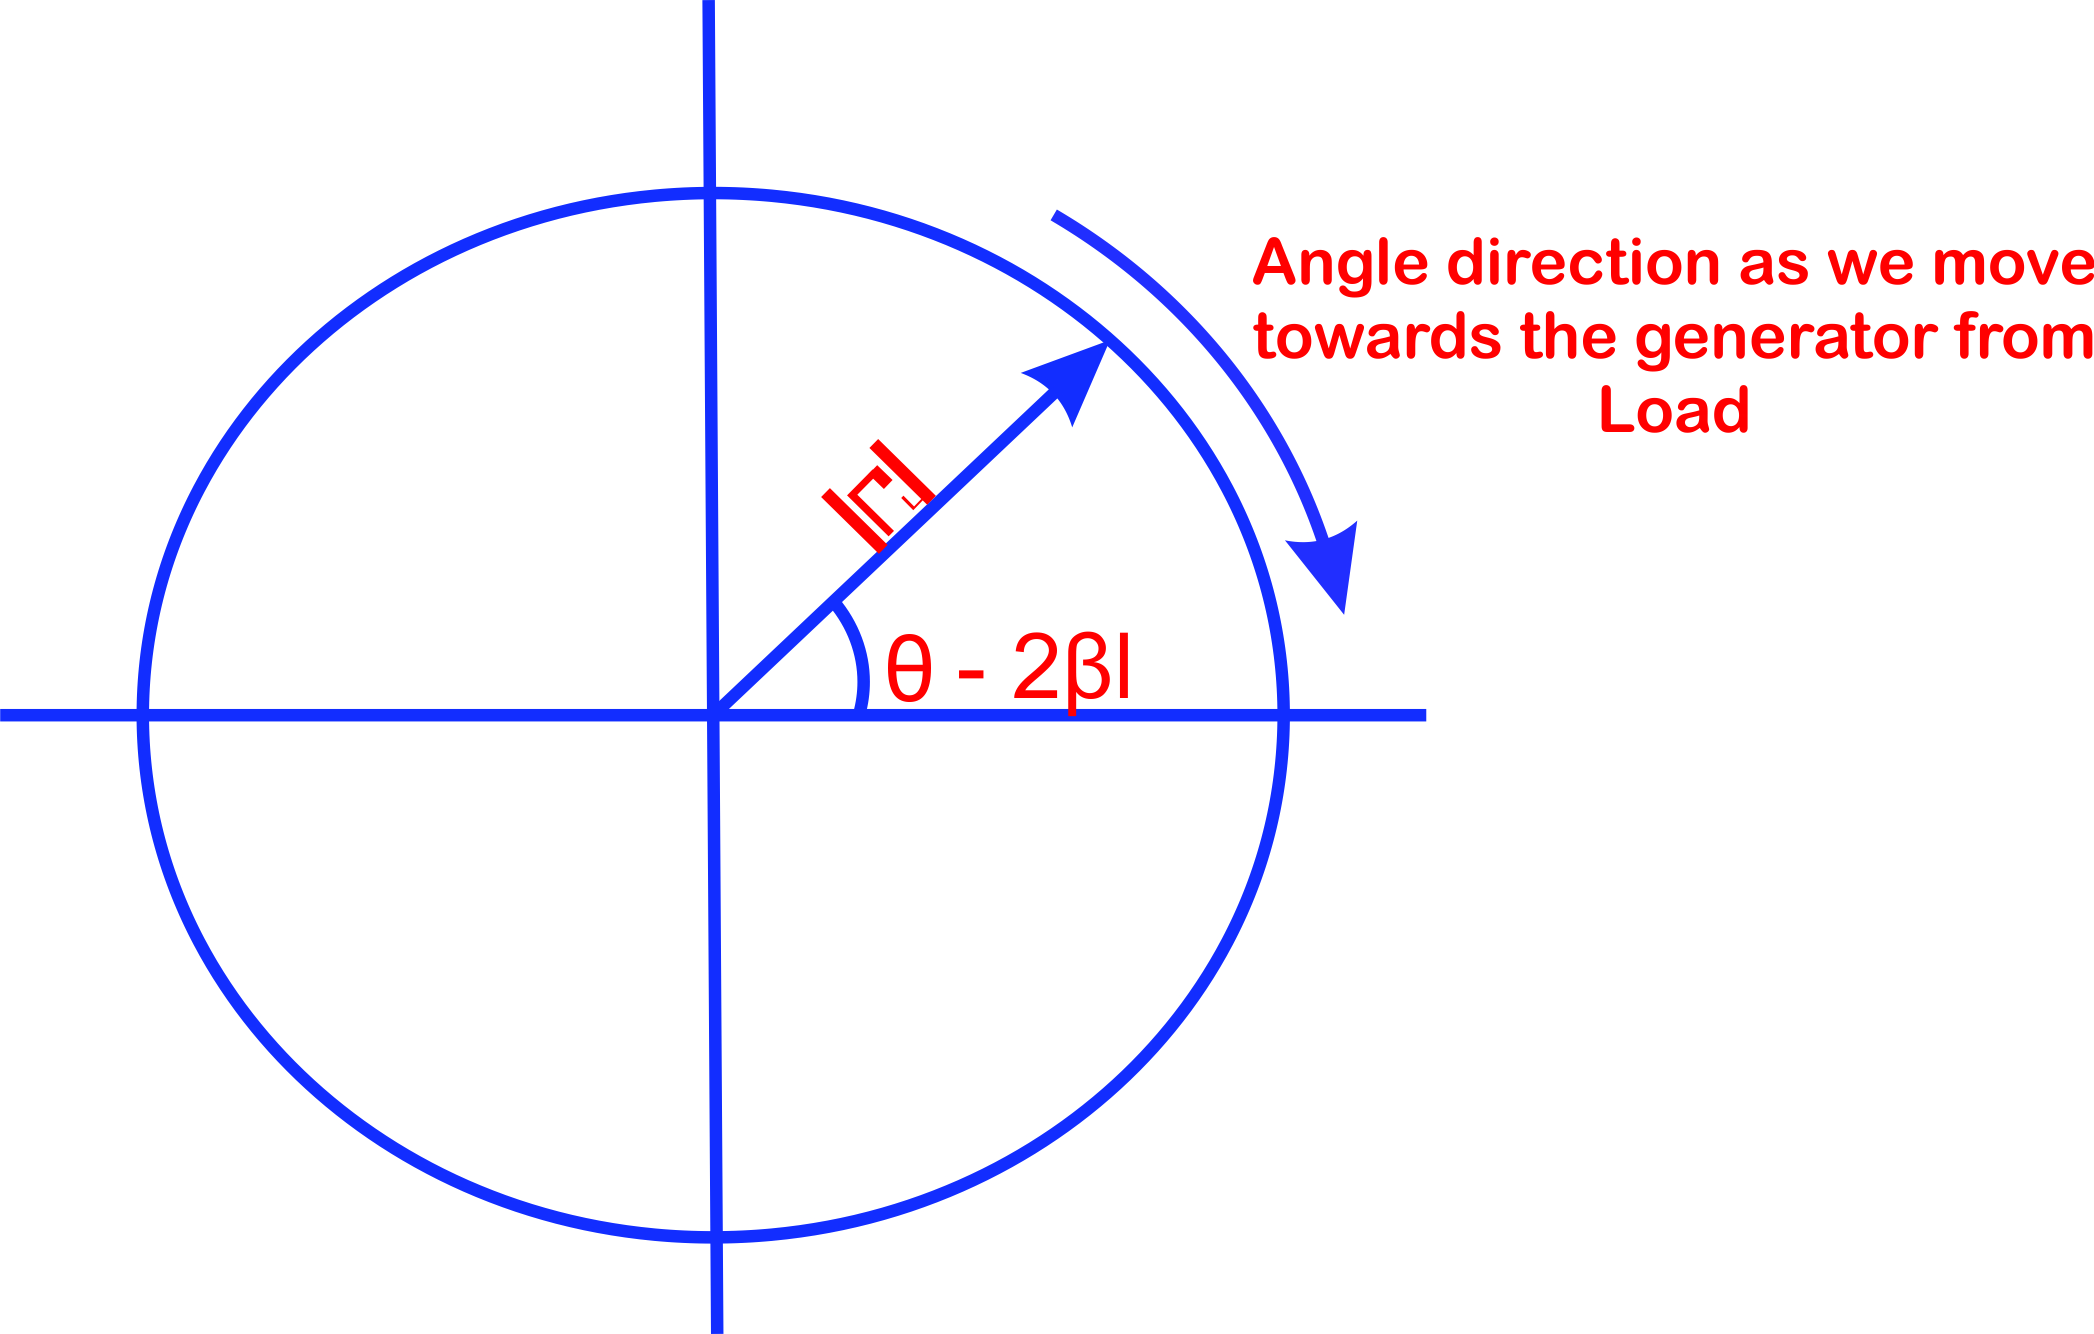
\includegraphics[width=0.7\linewidth]{./graphics/lkjhgryn}
\caption{Constant VSWR Circle}
\label{fig:lkjhgryn}
\end{figure}

Since $|\Gamma_L|$ is same at any point on the circle, then the VSWR is same for all points on the circle, hence we call the circle a constant VSWR circle. 
% Note that while solving transmission line problems, we have to draw constant VSWR circles on the Smith chart so the Smith chart readily gives the constant resistance and reactance circles in the limit circle of $|\Gamma_L|\leq 1$.
One should always note that the centre of all VSWR circles is same as that of the origin of  the complex gamma plane and the magntude of the reflection coefficient is always less or equal to 1. Larger radius of $|\Gamma_L|$ gives more reflection coefficient with lower impedance match and smaller radius of  $|\Gamma_L|$ gives smaller magnitude of reflection coefficient and a better impedance match (see figure~\ref{fig:poiuyfd}).

When we say that we have better impedance matching on the Smith chart, visually speaking, we mean that the point closest to the centre of the Smith chart is better for impedance matching because it represents a smaller magnitude of reflection coefficient. 

With the understanding of superimposing the constant VSWR circle on the Smith chart, we can therefore solve the transmission line problem.
\begin{figure}[h]
\centering
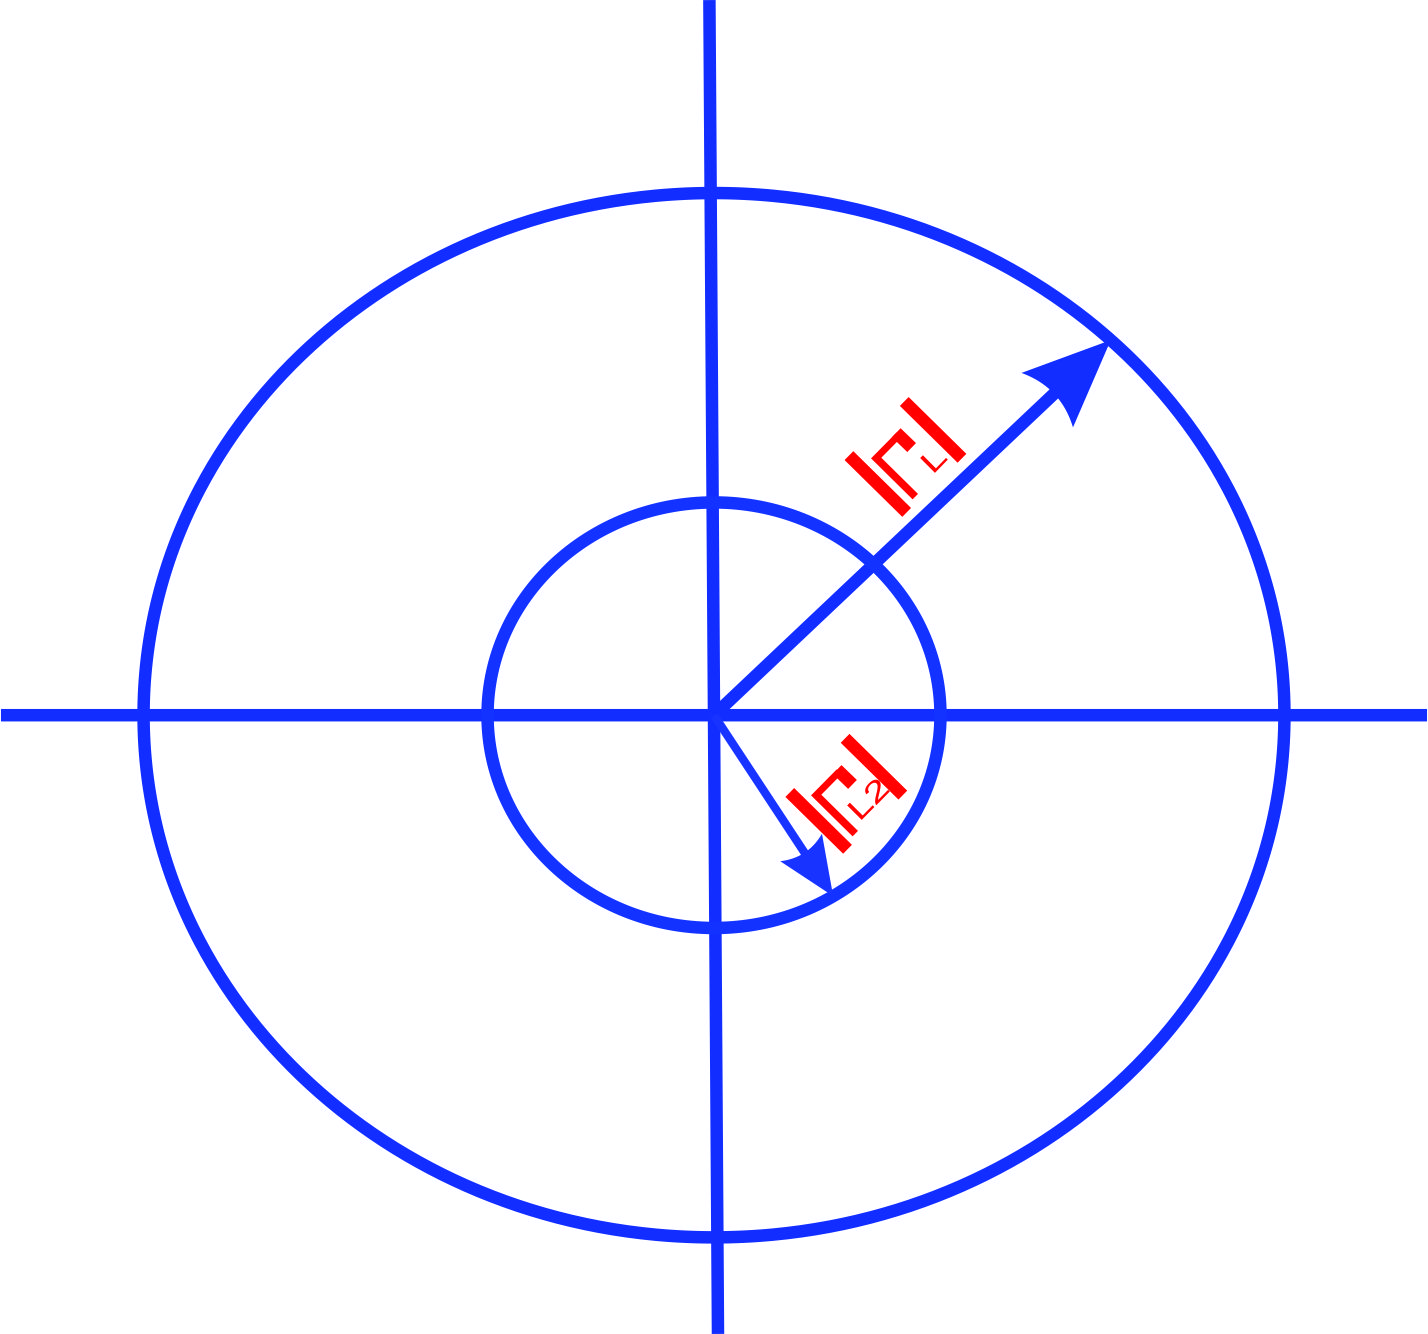
\includegraphics[width=0.57\linewidth]{./graphics/poiuyfd}
\caption{Impedance matching with different constant VSWR circles}
\label{fig:poiuyfd}
\end{figure}

\section{Transmission Line Analysis using Admittance}
However as we have said, you may have connections in transmission lines which are in the form of parallel connections and we know that from circuit analysis, anywhere we have parallel connections, it is easier to deal with admittances rather than impedances. Before now, we have been discussing load impedances and load characteristics impedance of transmission lines. However, if we have to make parallel connections on the transmission line, we represent the load as admittances and characteristics admittance before we carry out the analysis on the Smith chart. 

Thus, in this section, we will determine how the Smith chart is used when we compute in terms of admittances. Since the Smith chart gives the normalized impedances of the transmission line, the same thing will be derived for admittances so we shall first define the normalized admittance of the transmission line and for that, we would require what is called the \emph{characteristic admittance}\index{characteristics admittance} of the line. The characteristic admittance is given in equation~\eqref{eqn:characteristicsadmit}
\begin{equation}
Y_o = \frac{1}{Z_o}\label{eqn:characteristicsadmit}
\end{equation}
Then, normalizing the admittance would yeild
\begin{align*}
\bar{Y} = \frac{Y}{Y_o}\quad\text{thus, load admittance is }\quad\bar{Y}_L = \frac{Y_L}{Y_o}
\end{align*}
The reflection co-efficient as derived in equation~\eqref{eqn:refcoefficientfromload07} is given as
\begin{equation*}
\Gamma = \frac{Z - Z_o}{Z + Z_o} 
\end{equation*}
To determine the reflection coefficient in terms of admittance we replace the impedance $Z$ and characteristics impedance are then expressed as the inverse of admittance $\frac{1}{Y}$ and inverse of the characteristics admittance $\frac{1}{Y_o}$ respectively.
\begin{equation*}
\Gamma = \frac{\frac{1}{Y} - \frac{1}{Y_o}}{\frac{1}{Y} + \frac{1}{Y_o}}
\end{equation*}
We further simplify as follows;
\begin{dmath*}
\Gamma = \frac{Y_o - Y}{Y_o + Y}
= \frac{1 - \frac{Y}{Y_o}}{1 + \frac{Y}{Y_o}}
= \frac{1 - \bar{Y}}{1 + \bar{Y}} = -1\cdot\left(\frac{\bar{Y} - 1}{\bar{Y} + 1}\right)
\end{dmath*}
The negative sign indicates a phase change of 180\textdegree\footnote{
As -1 is a phase change of $\pi, e^{j\pi} = \cos\pi + j\sin\pi = -1$
} thus, it can be expressed as
\begin{equation}
\Gamma = \frac{\bar{Y} - 1}{\bar{Y} + 1}e^{j\pi}
\end{equation}
So the reflection coefficient written in terms of normalized admittances is same as reflection coefficient written in terms of normalized impedance except for the 180\textdegree\; phase change.

This implies that same value is derived for reflection coefficient when calculated using the normalized impedance or admittance except there is a phase shift of 180\textdegree\; that would be experienced on the transmission line. In other words, on the complex gamma plane of the Smith chart, the 180\textdegree\; phase shift will correspond to a rotation of 180\textdegree\; (see figure~\ref{fig:zstyuiou}). Essentially, the normalized impedance and admittance can be calculated in the same way except when carry out calculations for normalized admittances, there is a rotation of 180\textdegree\; on the complex gamma plane otherwise all other values and parameters remain unchanged.
\begin{figure}[h]
\centering
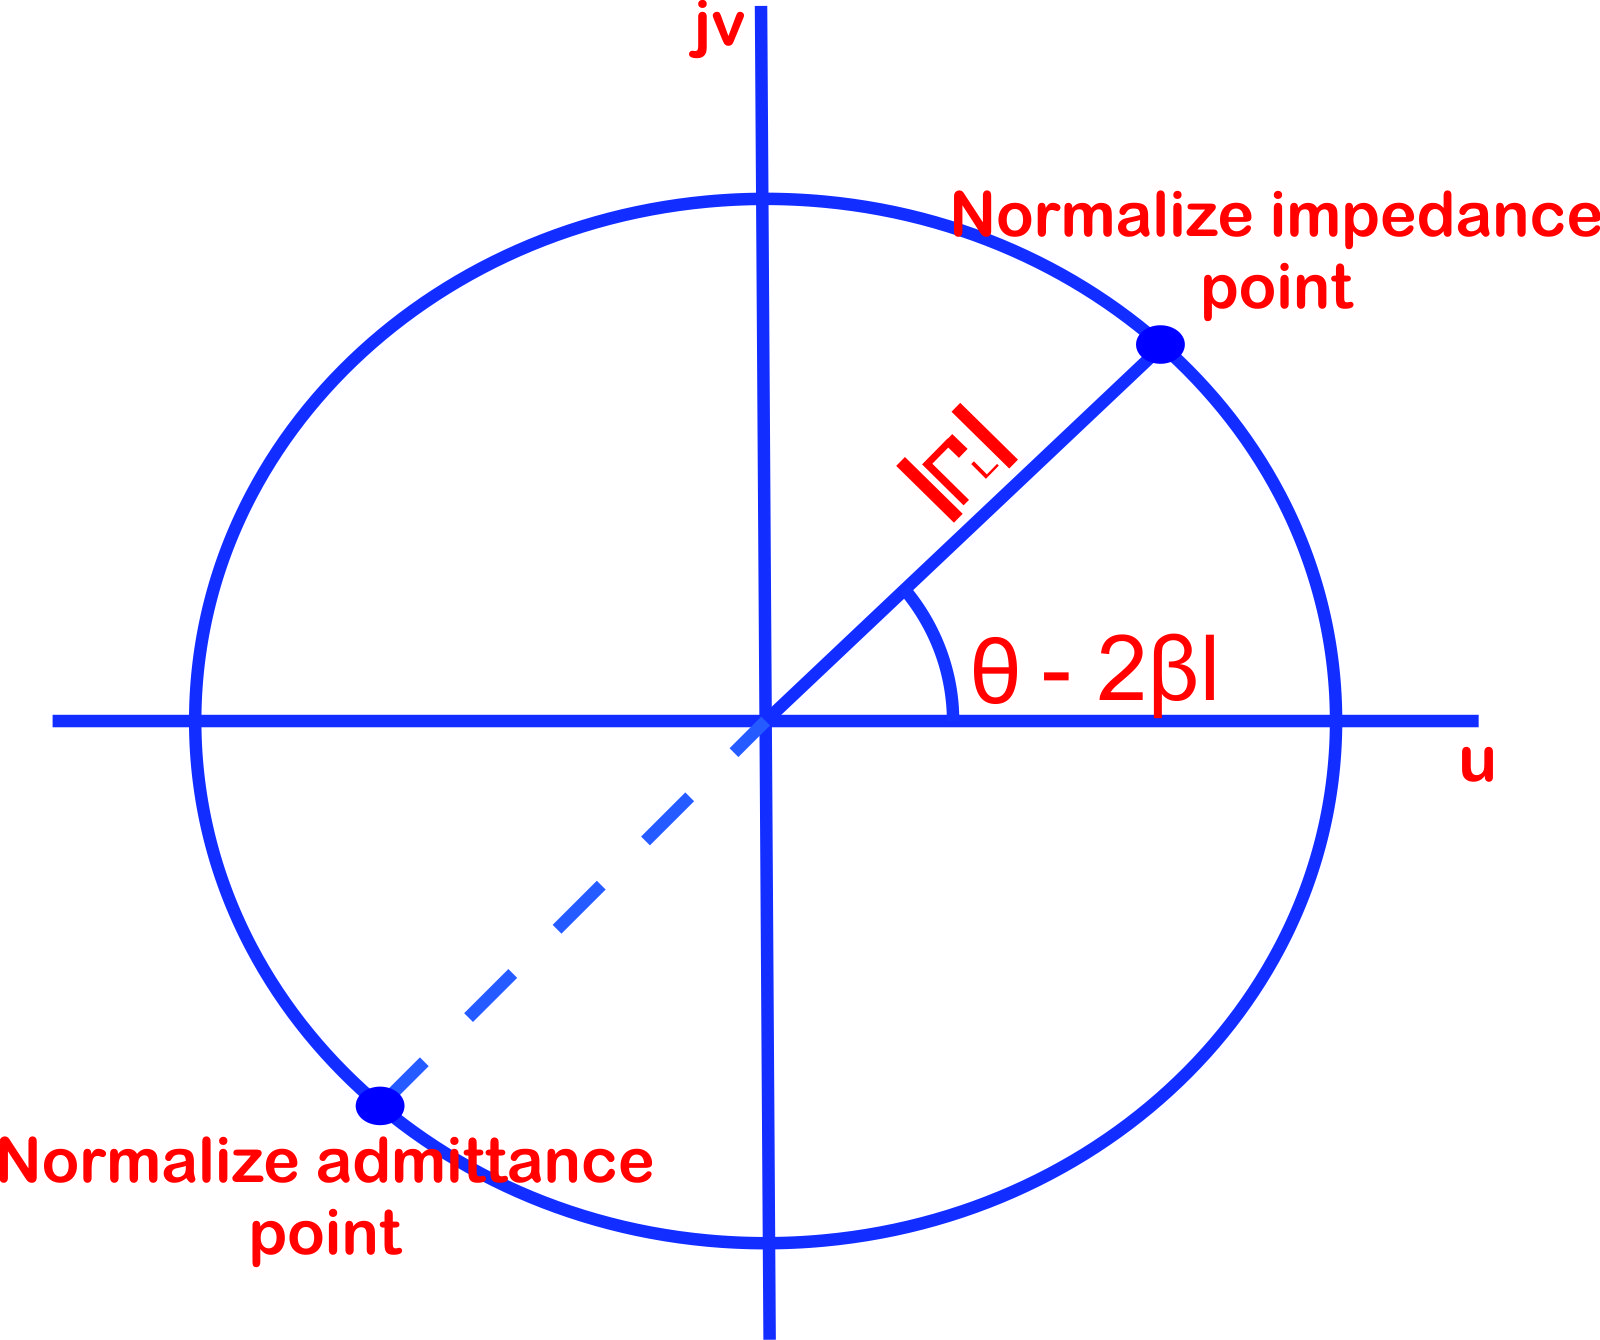
\includegraphics[width=0.6\linewidth]{./graphics/zstyuiou}
\caption{Impedance equivalent of Admittance on the gamma plane}
\label{fig:zstyuiou}
\end{figure}

Hence as far as the constant VSWR circles are concerned, any point on the Smith chart rotated by 180\textdegree\; corresponds to the normalized admittance with corresponding circles of constant resistance and circles of constant reactance. 

\emph{What would be the complex representation of the admittance?}
\begin{dmath*}
\bar{Y}=\frac{G + jB}{Y_o} = g + jb
= \text{conductance} + j (\text{susceptance})
\end{dmath*}
If we interchange $r$ with $g$ and $x$ with $b$, then the circles through the point on the constant VSWR circle will be the \textbf{circle of constant conductance} and the \textbf{circle of constant susceptance} which are similar to the circle of constant resistance and circle of constant reactance except that they are rotated by 180\textdegree\;. This implies that our analysis with admittances will resemble one where every point on the Smith chart is flipped and so the clustered end goes to the left hand side as shown in figure~\ref{fig:invertedsmithchart}.
\begin{figure}[h]
\centering
\includegraphics*[width=0.7\linewidth]{./graphics/smithchart1.jpeg}
\caption{Inverted Smith chart}\label{fig:invertedsmithchart}
\end{figure}

Alternatively, we can keep the Smith chart orientation the same and rotate the complex gamma axis by 180\textdegree\; before doing calculations for admittances. So, if we develop an understanding that we will not rotate the Smith chart, that means we want to use it in its original form, that is, the most clustered part of it to our right, then if we do the impedance calculations, the positive real axis is towards right and the positive imaginary axis goes up. However, during calculations using the Smith chart unchanged for admittances, the positive real axis is towards the left and the  positive imaginary axis will be downwards. Normally, whenever we do the Smith chart calculations, we do not rotate the Smith chart. For the impedance, the gamma axis is the  positive top right plane and for admittances, the bottom left plane is the positive plane. Depending on whether we are doing calculations for the impedance or admittances and if we require fixed measurement in the complex gamma plane, then the axis has to be rotated appropriately by 180\textdegree\; depending on whether we are using the impedance or admittance. This is important when finding the phase of the reflection coefficient, otherwise, the axis of the gamma plane is insignificant. So without worrying about the axis of the complex gamma plane, we can use the same Smith chart for the admittance as well as the impedance calculations. This is the reason why when you look at the Smith chart carefully, you will see that the upper half of the Smith chart is denoted by $(x,b)$ and the lower part $(-x,-b)$.The circles are denoted by either $r$ or $g$ so any normalized value of $r$ is equal to the same normalized value of $g$ which represent the same circle. 

Hence, as long we are dealing with a normalized quantity, the impedance and admittance can be treated exactly the same way on the Smith chart. However, the normalized values of $g$ and $r$ or $b$ and $x$ have different meaning physically. But do they represent the same physical conditions? The answer is NO! For example $r = 0; x = 0$, corresponds to a short circuit condition\textemdash\;the impedance is zero\textemdash\;however, if we take  a normalized value of admittance with $g=0, b=0$ which represents admittance equal to zero, it is not a short circuit but an open circuit condition on the line. Therefore, the normalized values of impedances and admittances can be treated exactly the same way in calculations but not the same interpretations for the physical conditions. In summary, mathematically, $g = 0\quad, b = 0\Longrightarrow$ open circuit and $g = \infty, b = \infty \Longrightarrow$  short circuit. 
\begin{figure}[h]
\centering
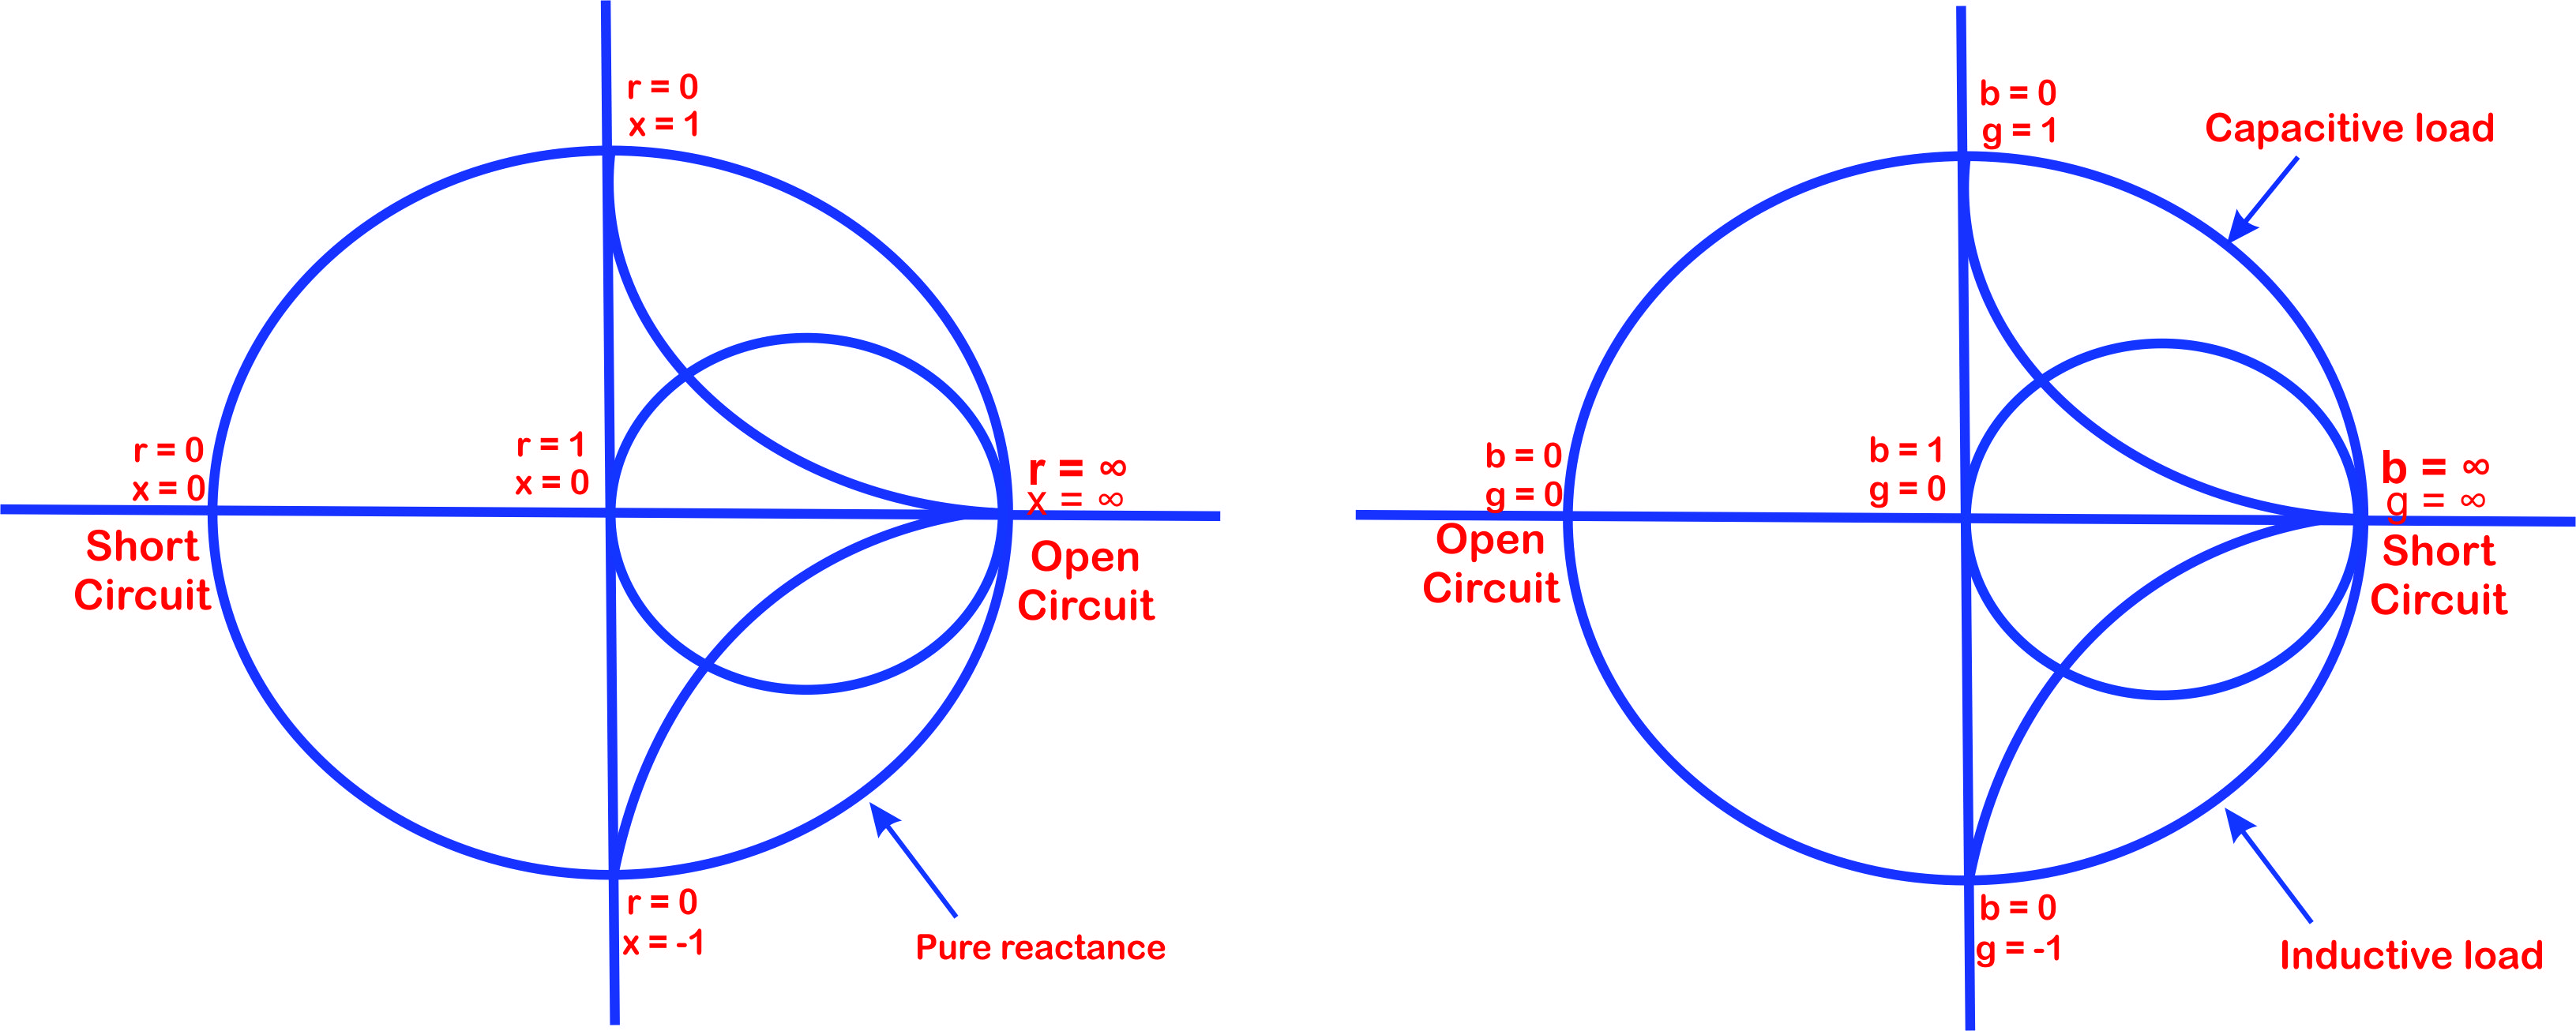
\includegraphics[width=1\linewidth]{./graphics/jnbkvfld}
\caption{Physical variation of impedance and admittance}
\label{fig:jnbkvfld}
\end{figure}

Let us therefore consider the points on Smith chart for the admittance where the special points $r$ and $x$ are replaced with $b$ and $g$ respectively. Maintaning the original orientation of the Smith chart then for the admittance Smith chart, the upper half of the Smith chart represents capacitive loads and the lower half represents the inductive loads (see figure~\ref{fig:jnbkvfld}). With these in mind, the use of Smith chart for impedance or admittance calculation is very straight forward.

Now lets make use of the Smith chart to solve transmission line problems. 

\section{Use of Smith chart for Transmission Line Calculation}
Let us consider the simplest problem we can think of for transmission line. Suppose for a given load, we want to find the reflection coefficient at the load point. Analytically, we can use the formula $\frac{Z_L - Z_0}{Z_L + Z_0}$ but in using the Smith chart, the problem is much simpler to solve. Remember the impedance and admittance you have on Smith chart are all normalized quantities. So we take the following steps

\subsection*{Procedure:}
\begin{enumerate}[(i)]
\item Normalize $Z_{L}$ to get $\bar{Z}_{L}$, that is, $\frac{Z_{L}}{Z_{0}}$.
\item Determine this point on the Smith chart, that is,  $r+jx$ by identifying the constant resistance and reactance circle with the value $r$ and $x$ respectively and the point of intersection (see figure~\ref{fig:lfds}).
\begin{figure}[h]
\centering
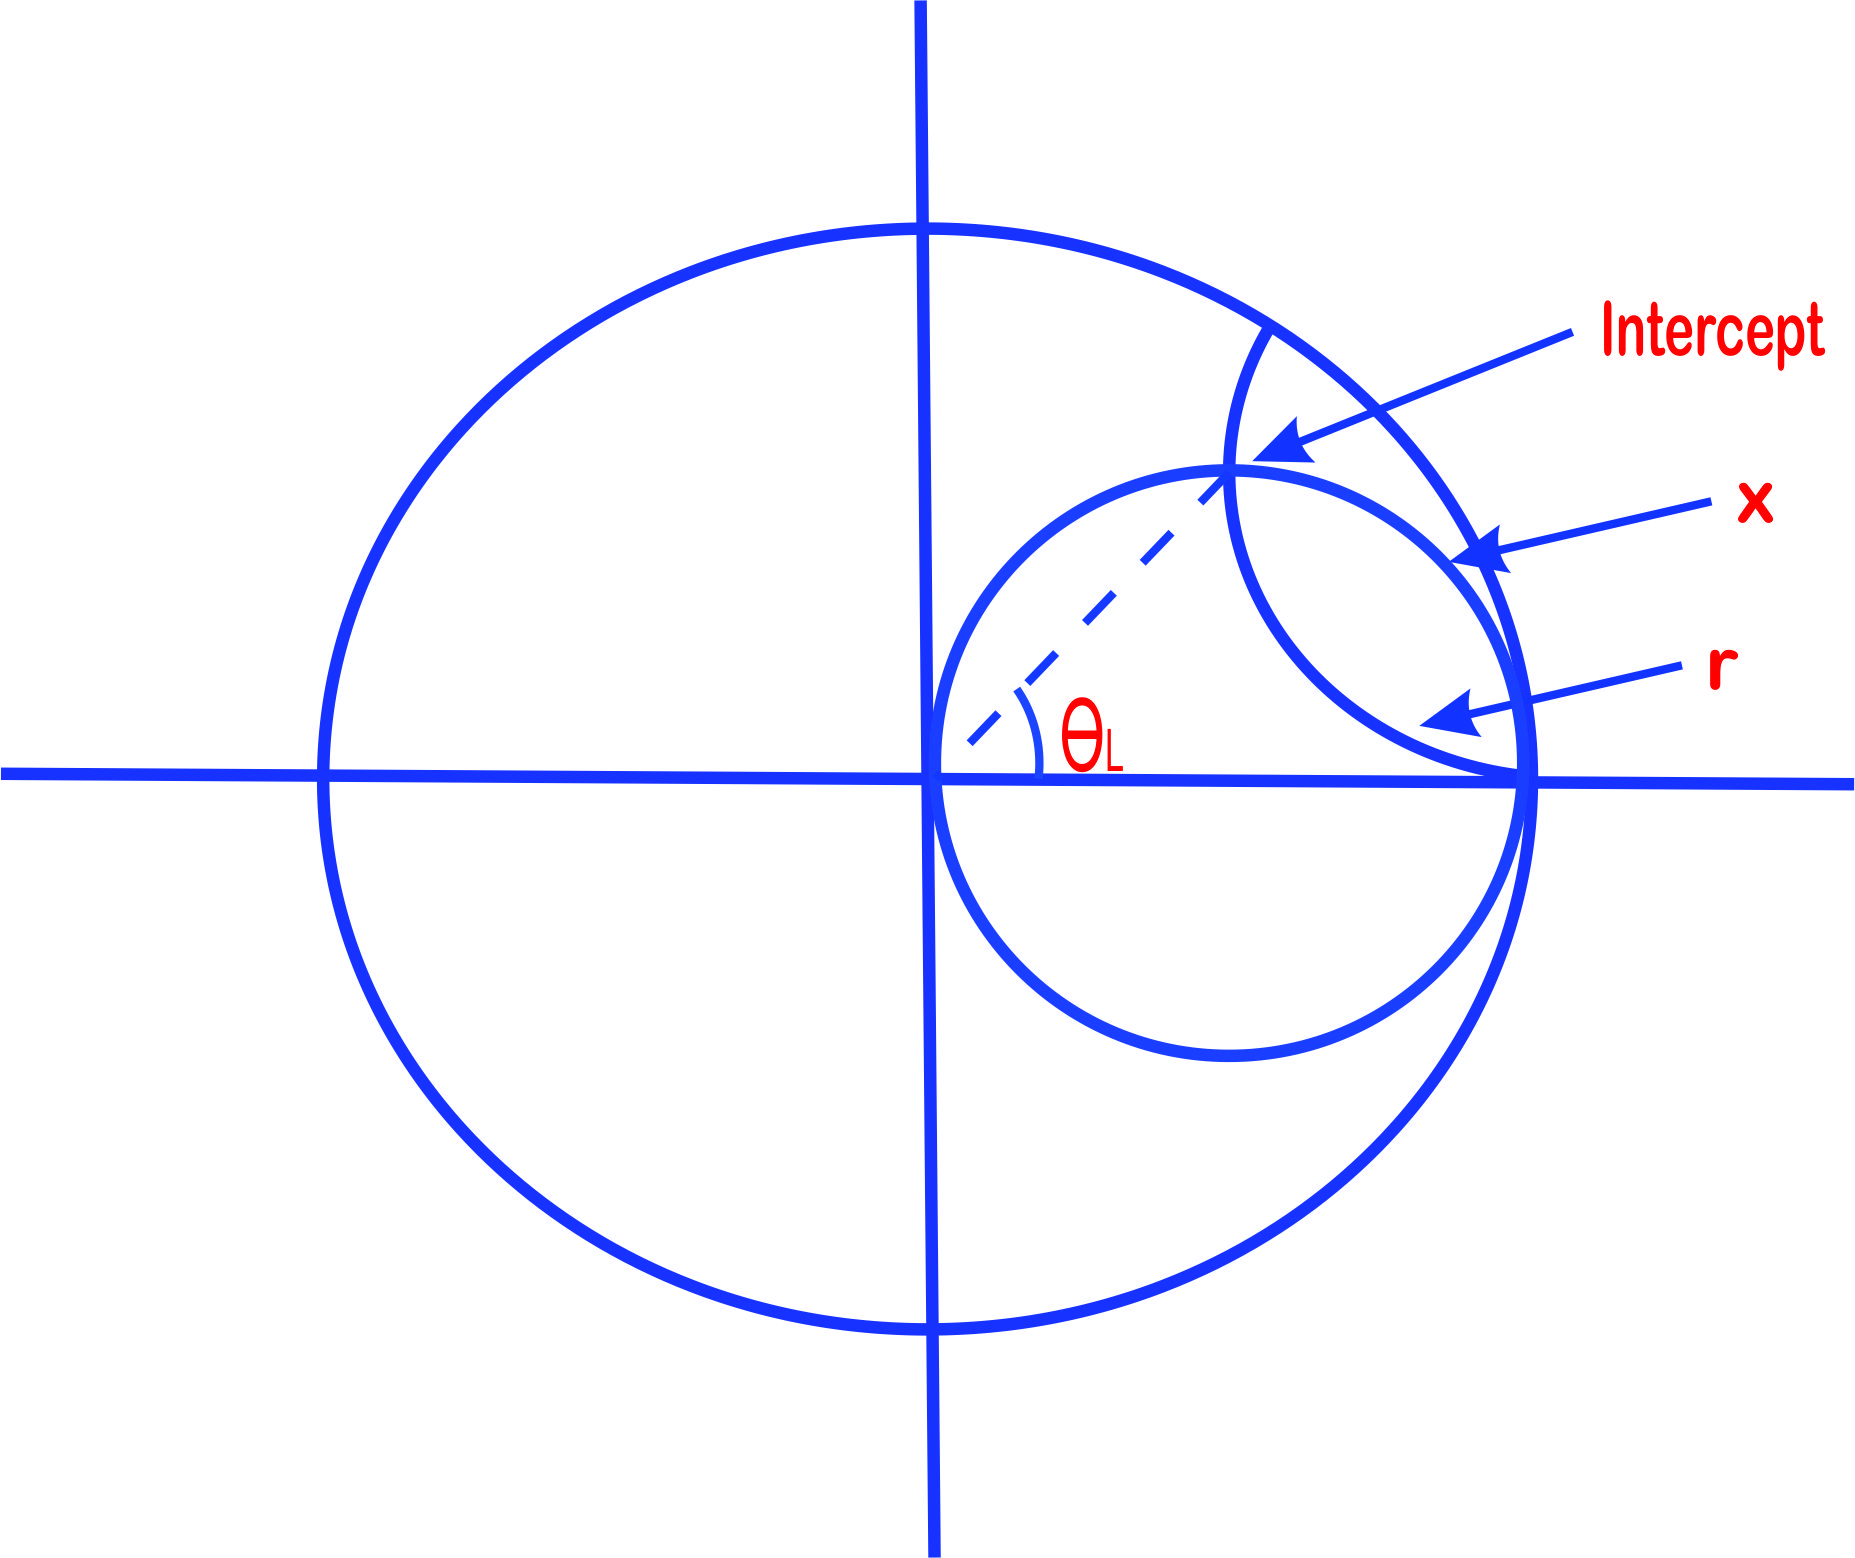
\includegraphics[width=0.7\linewidth]{./graphics/lfds}
\caption{Point of intersection of circles of constant resistance and reactance}
\label{fig:lfds}
\end{figure}

\item Determine the distance of the point of intersection from the origin to find the magnitude of the reflection coefficient, $|\Gamma_L|$ and then the corresponding phase given as $\theta_L$.
\end{enumerate}

So without doing any calculation, just by measuring its distance, and the angle, we get the magnitude of reflection coefficient, $|\Gamma_L|$
and phase angle, $\theta_L$. 

Similarly, for the admittance, let $\bar{Y} = g + jb$. We determine the point of intersection on the Smith chart the same way as that of impedance, however, to find out the complex reflection coefficient, maintaining the orientation, then the positive real axis is to the left. So the phase angle will be measured from the positive real axis as shown in figure~\ref{fig:kjhgfds}. We summarize the steps as follows.
\begin{figure}[h]
\centering
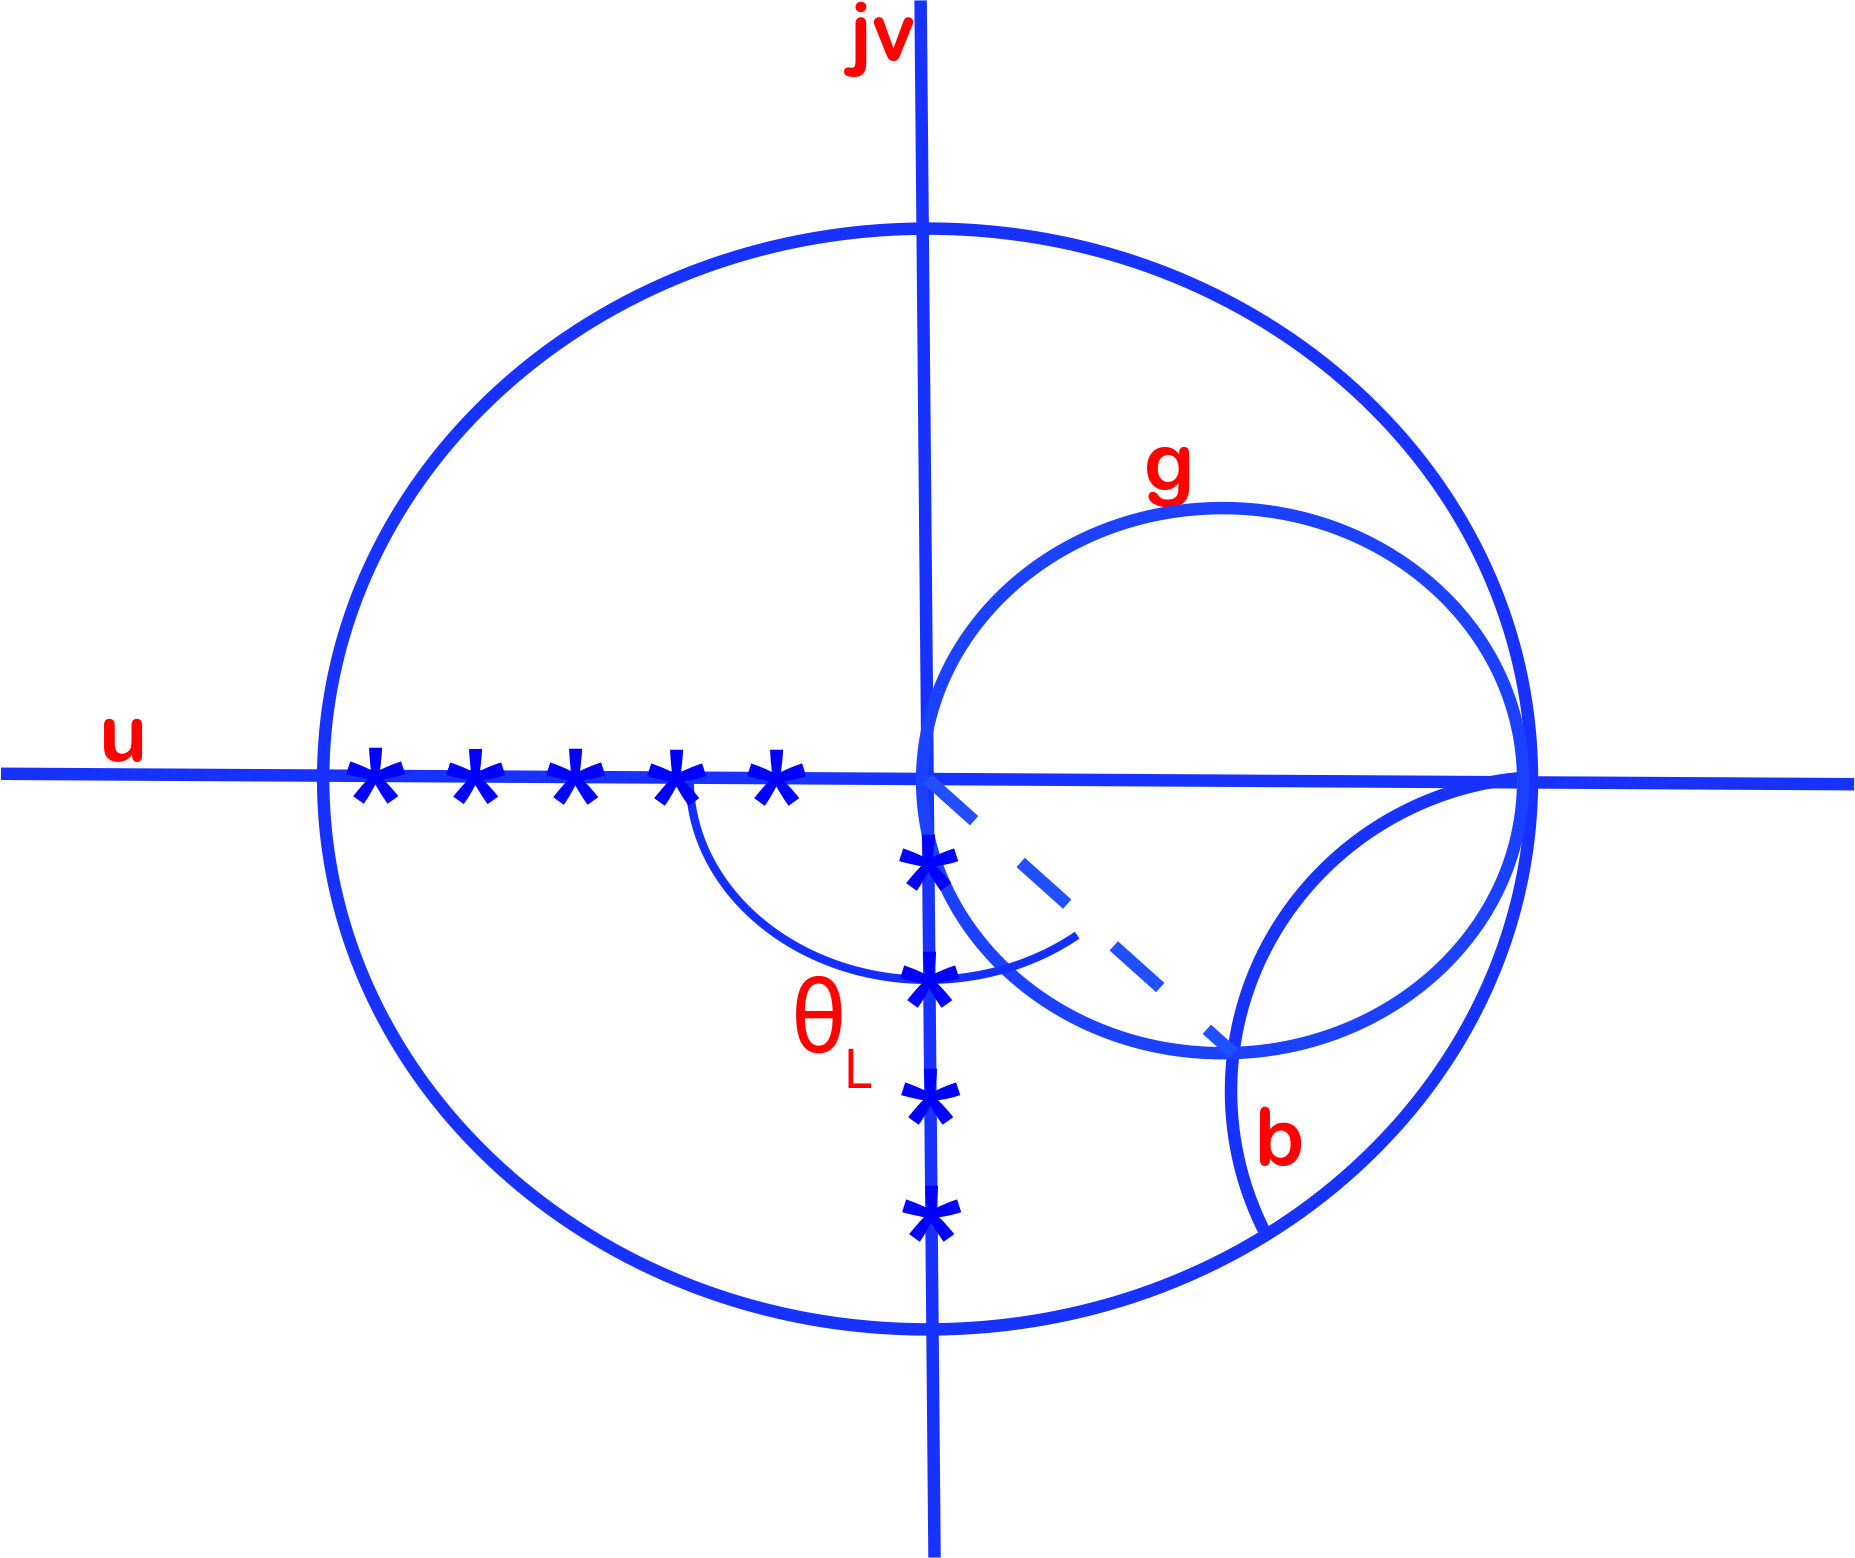
\includegraphics[width=0.7\linewidth]{./graphics/KJHGFDS}
\caption{Determining the reflection coefficient for admittance on a Smith chart}
\label{fig:kjhgfds}
\end{figure}

\subsection*{Procedure:}
\begin{enumerate}[(i)]
\item Normalize the admittance $\bar{Y}$ with the characteristic admittance, $Y_o$.
\item Determine the point on the Smith chart which is the point of intersection of the circle of constant conductance, $g$ and the circle of constant susceptance, $b$.
\item Determine the distance of the point from origin to find the magnitude of the reflection coefficient,  $|\Gamma_L|$ but the phase angle, $\theta_L$ will be measured from the  positive real axis (see figure~\ref{fig:kjhgfds}). 
\end{enumerate}

Thus, when we are using normalized impedance or admittance, appropriate rotation has to be made on the coordinate axes of the Smith chart. Once this is done, the calculation of the complex reflection coefficient is very straight forward. Mark the normalized points on the Smith chart. Find the distance from the origin to the marked point and then measure the angle from this marked point from the positive real axis which differs for impedance and admittance while maintaining the orientation of the Smith chart. 

In another simple transmission line problem, let us suppose the magnitude of the reflection coefficient and phase angle is given, but we need to find the load. The steps are summarized below.
\subsection*{Procedure:}
\begin{enumerate}[(i)]
\item Draw a cirle of radius equal to the magnitude of the reflection coefficient from the origin.
\item Determine phase angle from the positive real axis depending on whether the impedance or admittance value at the load is required.
\item Mark the point on the circle and find the corresponding $r$ and $x$ circles or $g$ and $b$ circles.
\item Multiply the normalized impedance or admittance by the characteristic impedance or admittance to get the load impedance or admittance.
\end{enumerate}

\subsection{Impedance Transformation}
A common problem in transmission line is impedance transformation. We have shown how it is done analytically but \emph{how can we perform impedance transformation graphically?} 
\begin{figure}[h]
\centering
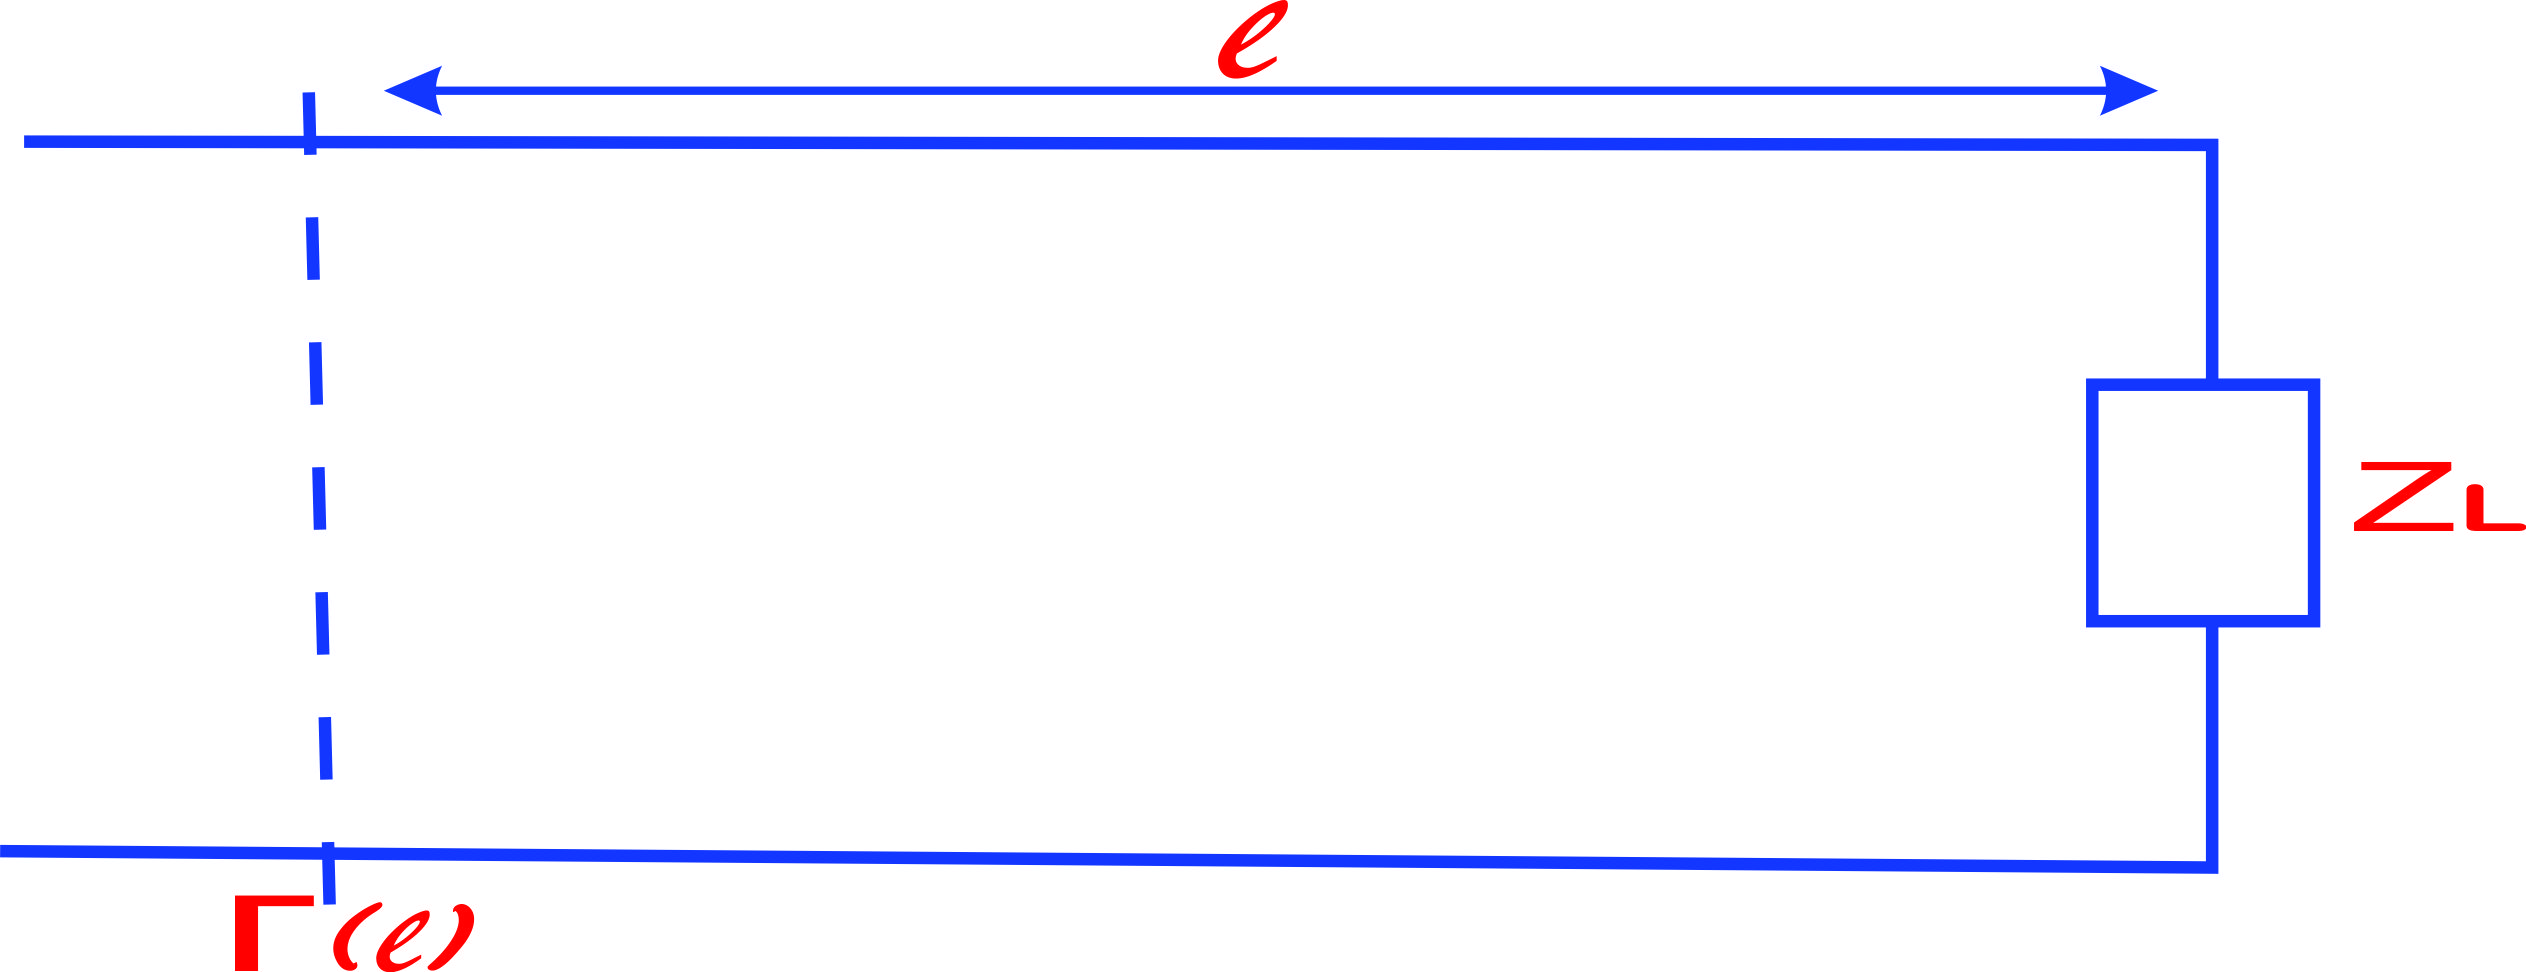
\includegraphics[width=0.7\linewidth]{./graphics/wertuyuk}
\caption{Tranformed impedance at distance $l$ from the load}
\label{fig:wertuyuk}
\end{figure}

If the load impedance is given as shown in figure~\ref{fig:wertuyuk} and we are asked to find the reflection coefficient and load impedance at another point $l$ on the transmission line, that is, given $Z_L$ or $Y_L$, we are to find $Z_L$ or $Y_L$ at distance $l$ from the load. We will use a hypothetical sketch of the Smith chart shown in figure~\ref{fig:uytrewsxcvbj}.
\begin{figure}[h]
\centering
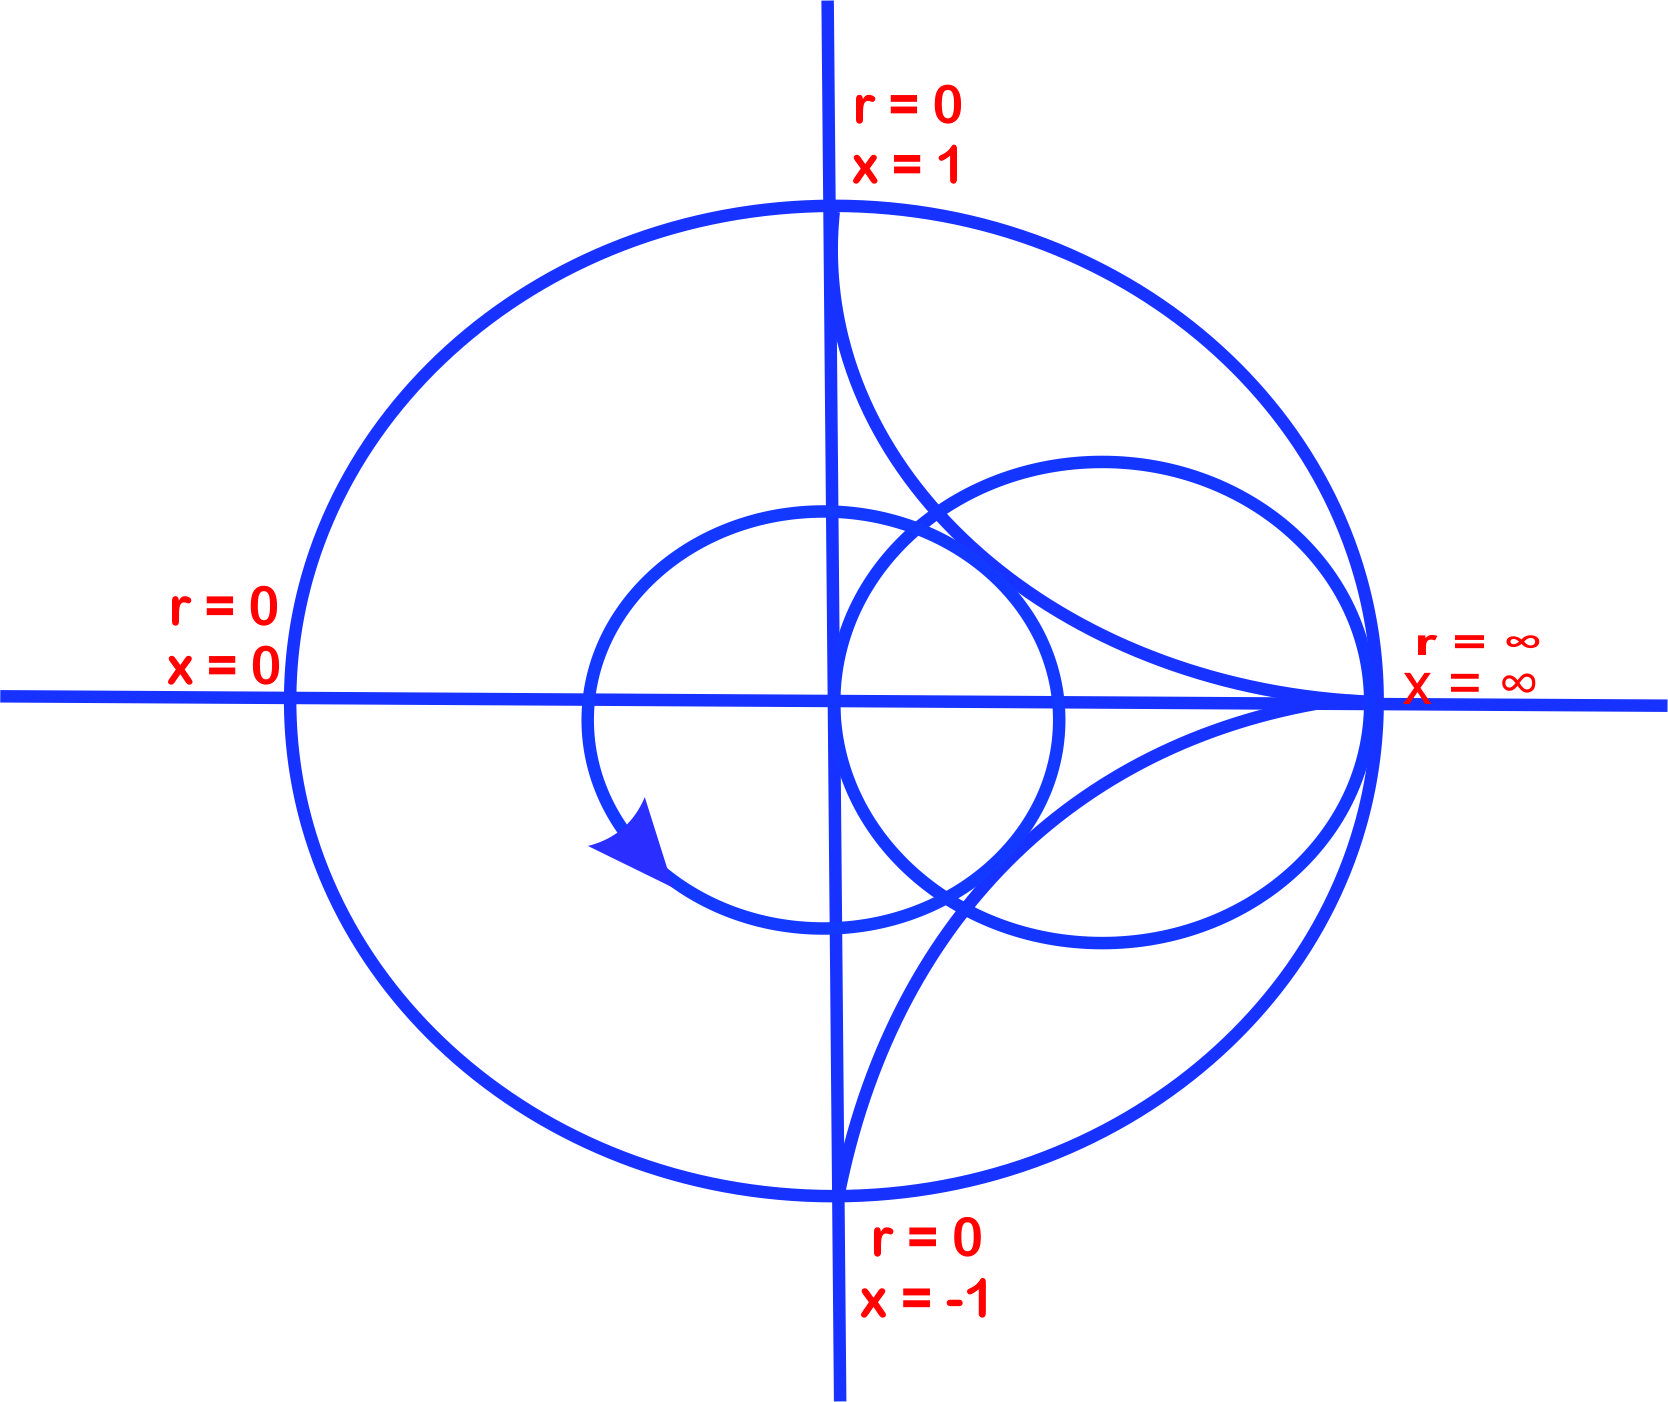
\includegraphics[width=0.9\linewidth]{./graphics/uytrewsxcvbj}
\caption{Points along the constant r and x Circles}
\label{fig:uytrewsxcvbj}
\end{figure}

\subsection*{Procedure:}
\begin{enumerate}[(i)]
\item If the impedance is not normalized, we normalize all impedances.
\item Determine the point, $\bar{Z}_L$, on the Smith chart and draw a circle passing through the point from the origin. As we have seen earlier, the magnitude of the reflection coefficient remains same as the point moves on the circle which is a constant VSWR circle.
\item Determine the point that translates to a distance $l$. In a Smith chart, one rotation, $2\pi$ translate to a phase change of $2\beta{l}$\footnote{
As we move along the transmission line, the phase angle changes by $2\beta{l}$ in the clockwise direction (from load towards generator).
}, that is $2\beta{l} = 2\pi\Longrightarrow l = \frac{\pi}{\beta} = \frac{\lambda}{2}$\footnote{
$\beta = \frac{2\pi}{\lambda}$
} (see figure~\ref{fig:mjhtre}). Therefore, a full rotation around the Smith chart corresponds to a distance of $\frac{\lambda}{2}$ on a constant VSWR circle\footnote{
The above analysis makes sense since one characteristics of the transmission line is that it's impedance characteristics repeats every $\frac{\lambda}{2}$ distance on the line.
}. So we determine the corresponding $x\lambda$ for the value of $l$ moving clockwise along the VSWR from the point $\bar{Z}_L$.
\begin{figure}[h]
\centering
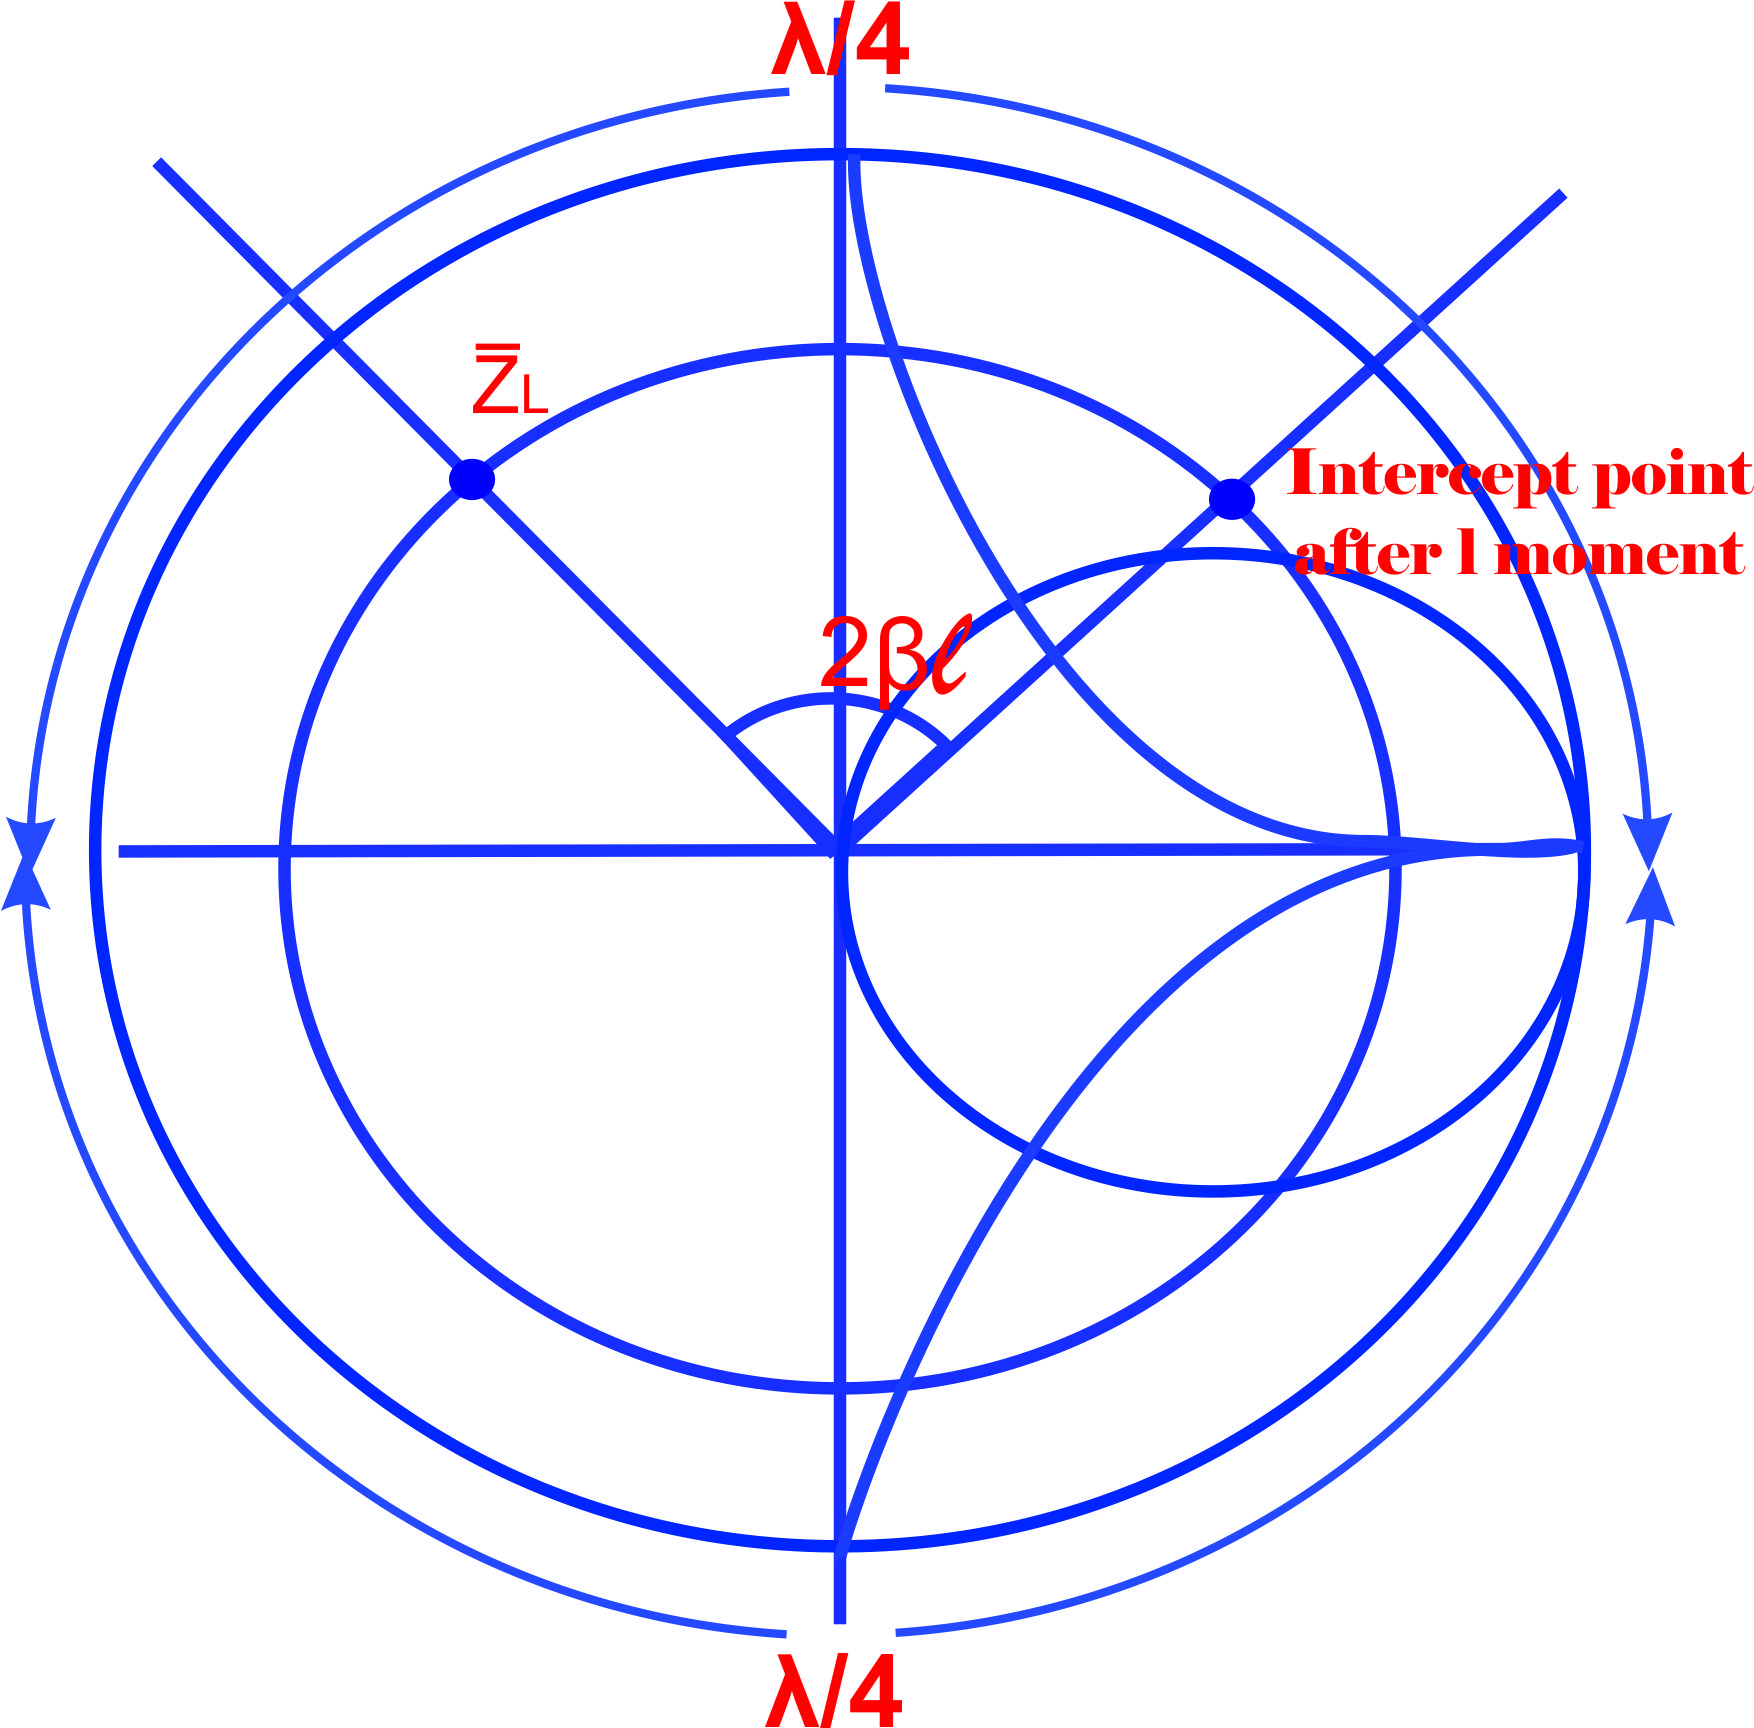
\includegraphics[width=0.7\linewidth]{./graphics/mjhtre}
\caption{Tranformed impedance at distance $l$ from the load}
\label{fig:mjhtre}
\end{figure}

\item Mark the new point on the Smith chart and determine the magitude of the reflection coefficient and phase angle as shown in figure~\ref{fig:uyhbgjvkclxse} or the circle of constant resistance and circle of constant reactance to determine the normalized impedance at $l$, that is, $\bar{Z}_{l} = r + jx$.
\begin{figure}[h]
\centering
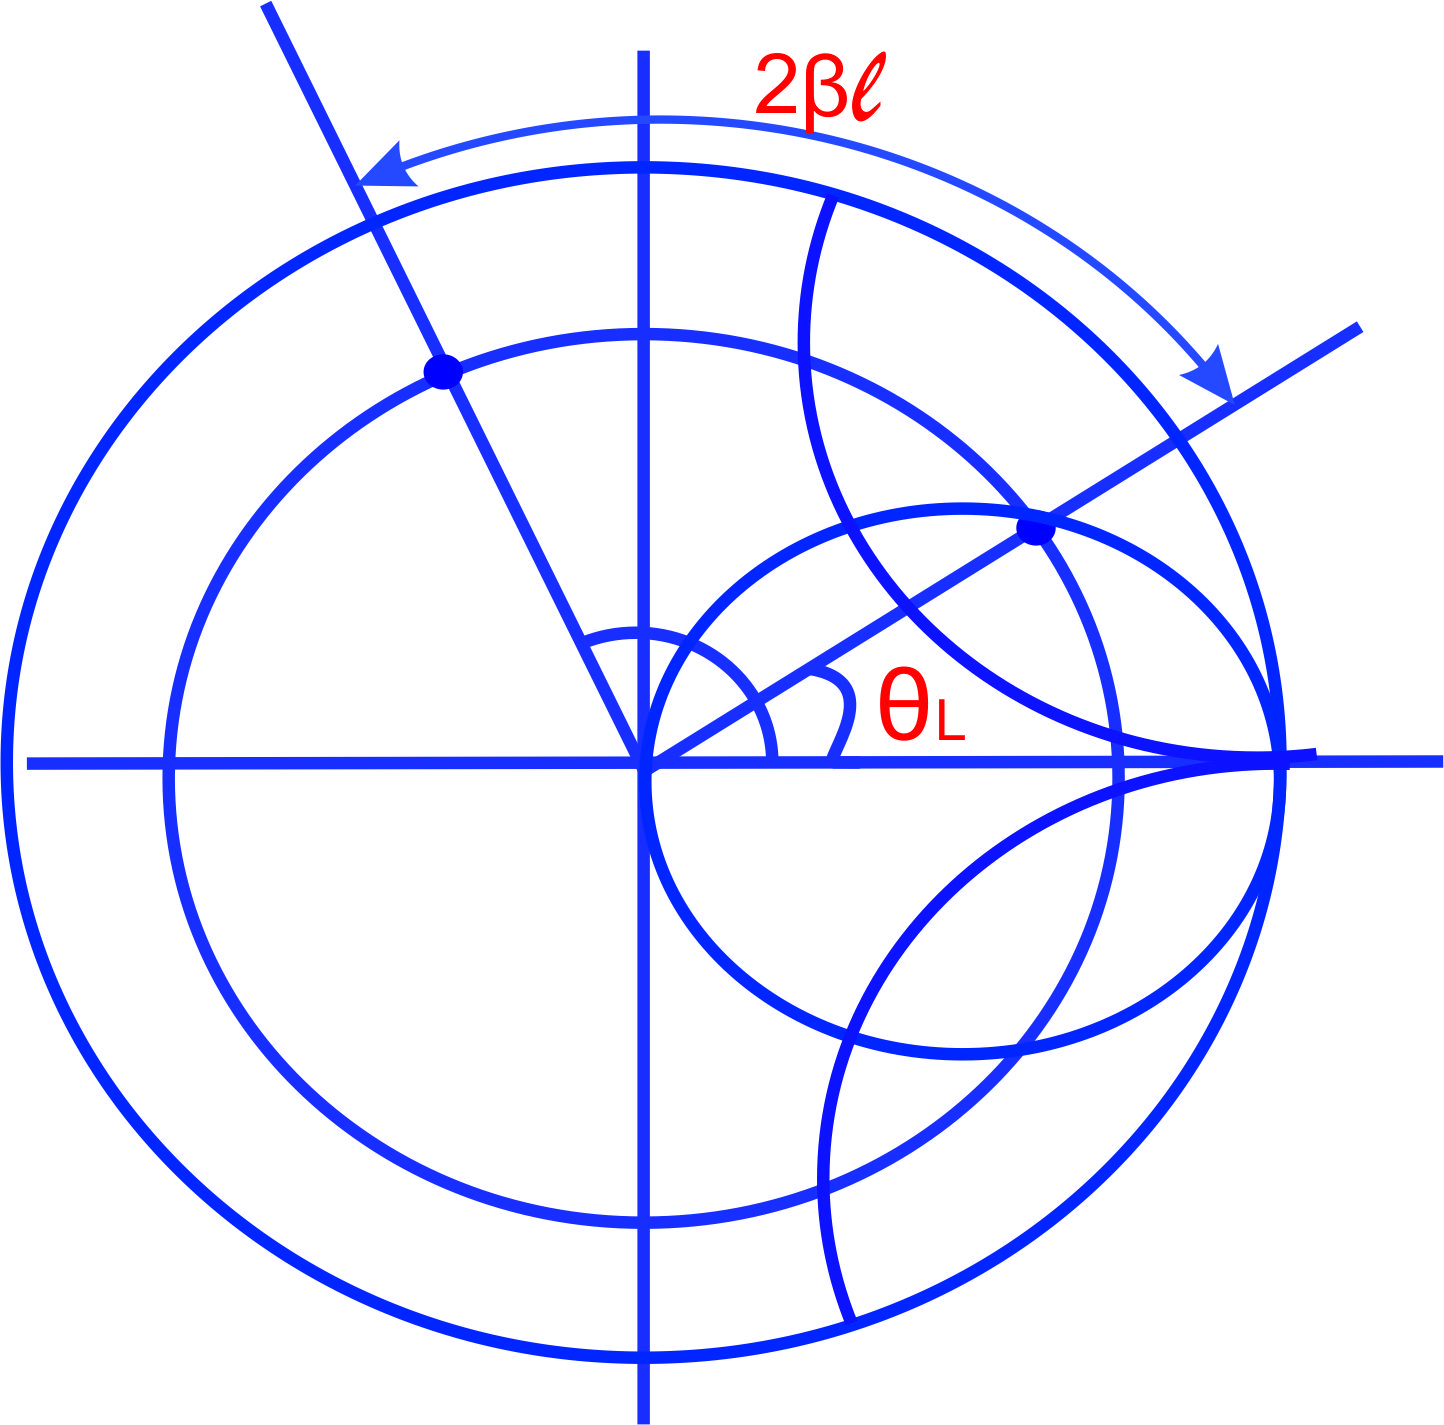
\includegraphics[width=0.7\linewidth]{./graphics/uyhbgjvkclxse}
\caption{New phase angle after rotation}
\label{fig:uyhbgjvkclxse}
\end{figure}

\item Multiply the normalized impedance at $l$ by the characteristic impedance $Z_o$ to get $\bar{Z}_{l}$ at the new location.
\end{enumerate}

A more general overview of a transmission problme is one where the impedance is given at a particular location and we need to transform the impedance to another location. If the new location is to the left of the previous impedance (towards the generator) then we follow the aforementioned steps, otherwise we reverse the direction of the angular rotation instead of $-2\beta{l}$, we have $+2\beta{l}$ which is counter-clockwise rotation. Hence, moving towards generator will be clockwise rotation and moving away from generator will be anti-clockwise rotation. The sense of rotation in impedance calculations is extremely important because that tells us whether to move towards the generator or away from the generator. Therefore, in all transmission line calculations, the direction of the generator should be given much consideration because that will decide the movement along the transmission line.

For admittance calculations, the same steps apply except in the sense of the position of the positive real axis (see figure~\ref{fig:dfyui}).
\begin{figure}[h]
\centering
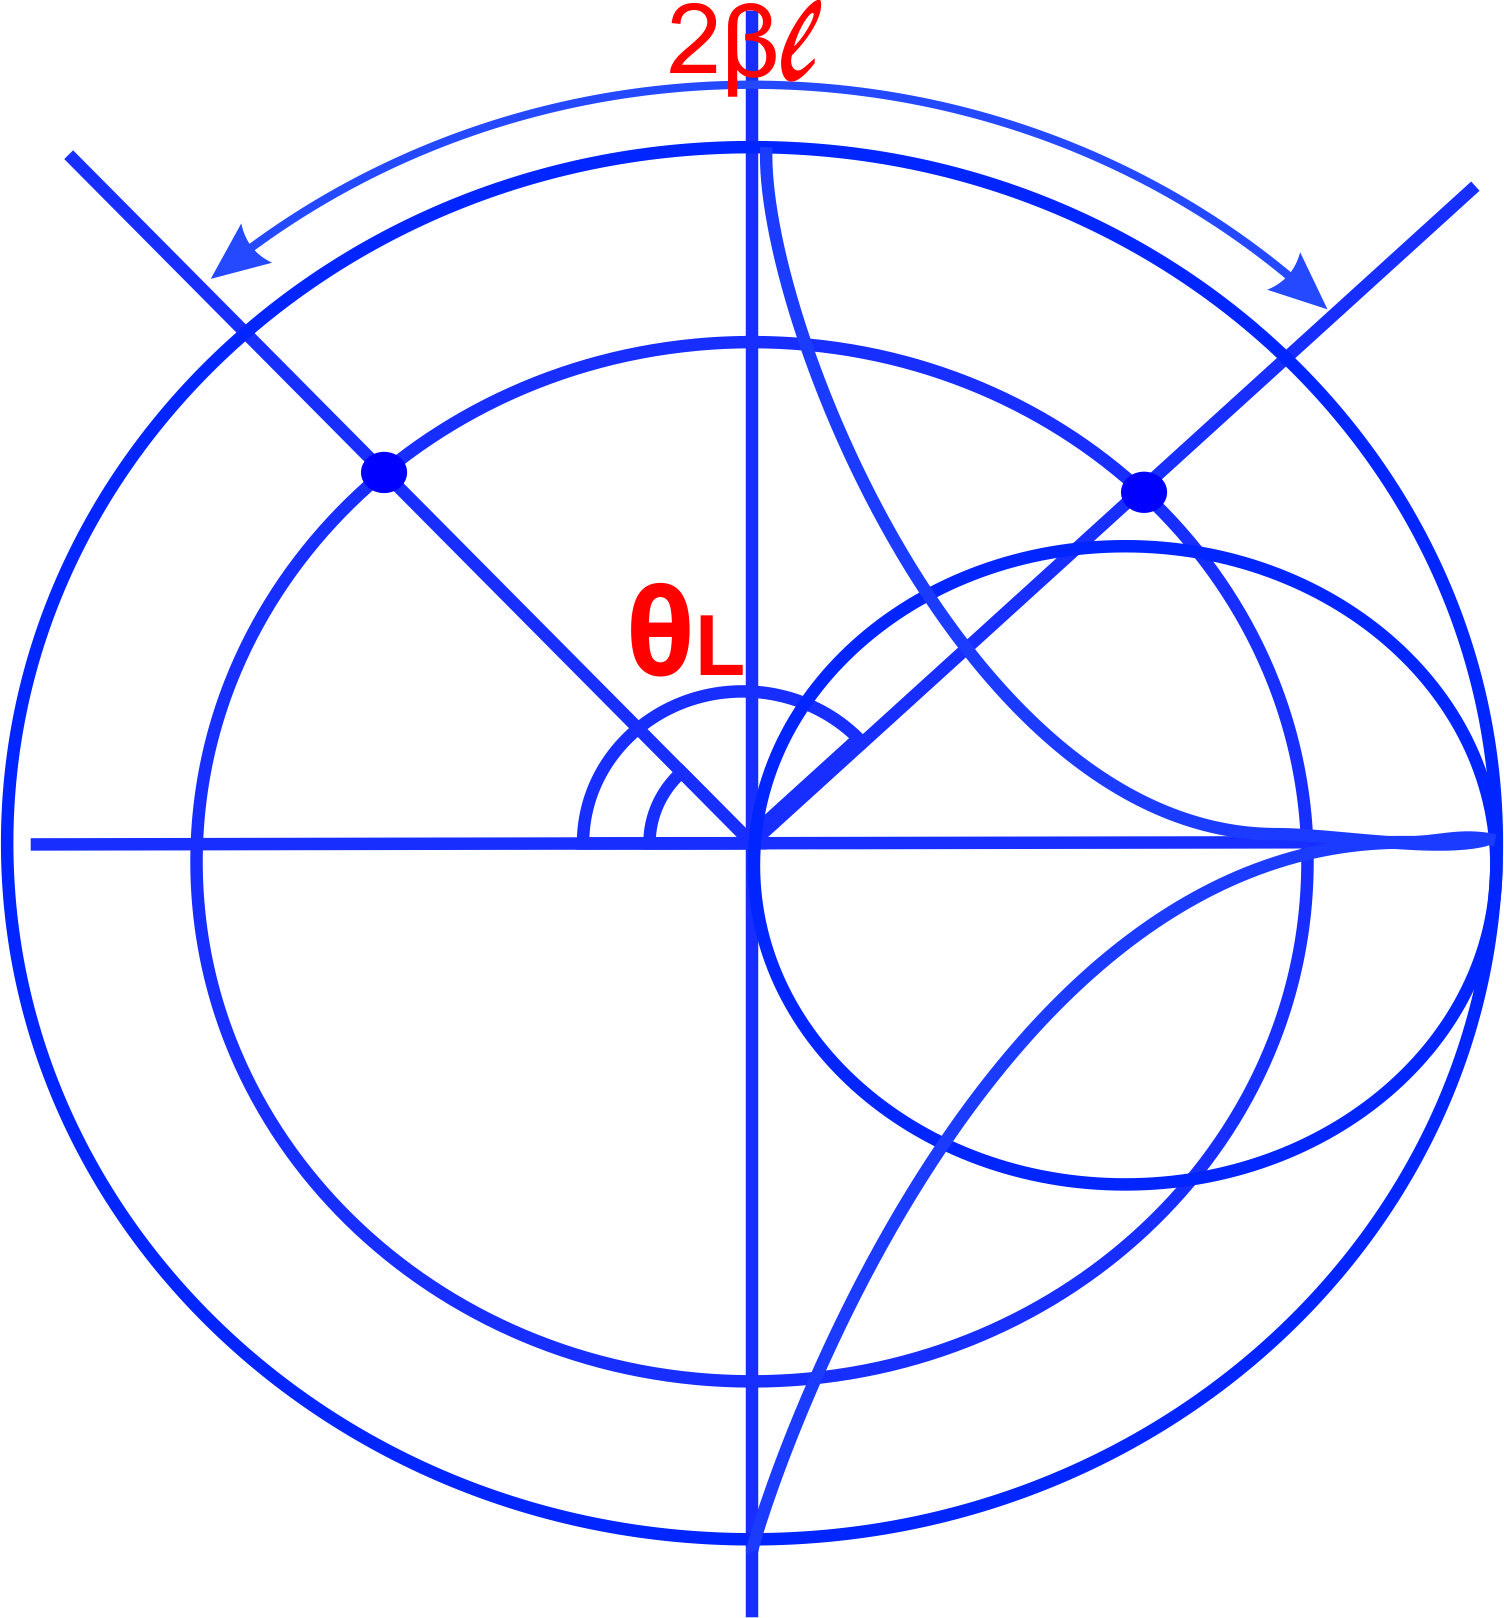
\includegraphics[width=0.7\linewidth]{./graphics/dfyui}
\caption{Phase angle measurement with admittance Smith chart}
\label{fig:dfyui}
\end{figure}

Analytically, the impedance transformation requires the calculation of sine and cosine functions that are unusually very complicated. With the help of the Smith chart, the impedance transformation is easily achieved.

\subsection{Voltage Standing Wave Ratio (VSWR)}
Another quantity which is a measure of reflection is the VSWR and we established previously that $R_\max = Z_{o}\rho$ and $R_\min = \frac{Z_o}{\rho}$. If we normalize $R_\max$ and $R_\min$ then we get:
\begin{equation}
\bar{R}_\max = r_\max = {\rho}
\end{equation}
and
\begin{equation}
\bar{R}_\min = r_\min = \frac{1}{\rho}
\end{equation}
Therefore, the maximum normalized resistance, $r_\max$ gives the VSWR, $\rho$. Similarly, on the left side of VSWR circle on the Smith chart we have $r_\min$. Hence $r_\min = \frac{1}{\rho}$. Thus, \emph{how do we determine the VSWR graphically?} On the real axis, we have only resistance and no reactance so points of intersection of the constant VSWR circle with the real axis gives the maximum and minimum normalized resistance (see figure~\ref{fig:oijhgfdsa}).  The reason why we call it the constant VSWR circle is because as determined in equation~\eqref{eqn:vswr}, it is given as $\frac{1 + |\Gamma|}{1 - |\Gamma|}$ which is constant for a lossless transmission line and these values of $r_\max$ and $r_\min$ can easily be deduced from the VSWR circles without a need to calculate. The VSWR is taken as the ratio of maximum impedance on the line to characteristics impedance.
\begin{figure}[h]
\centering
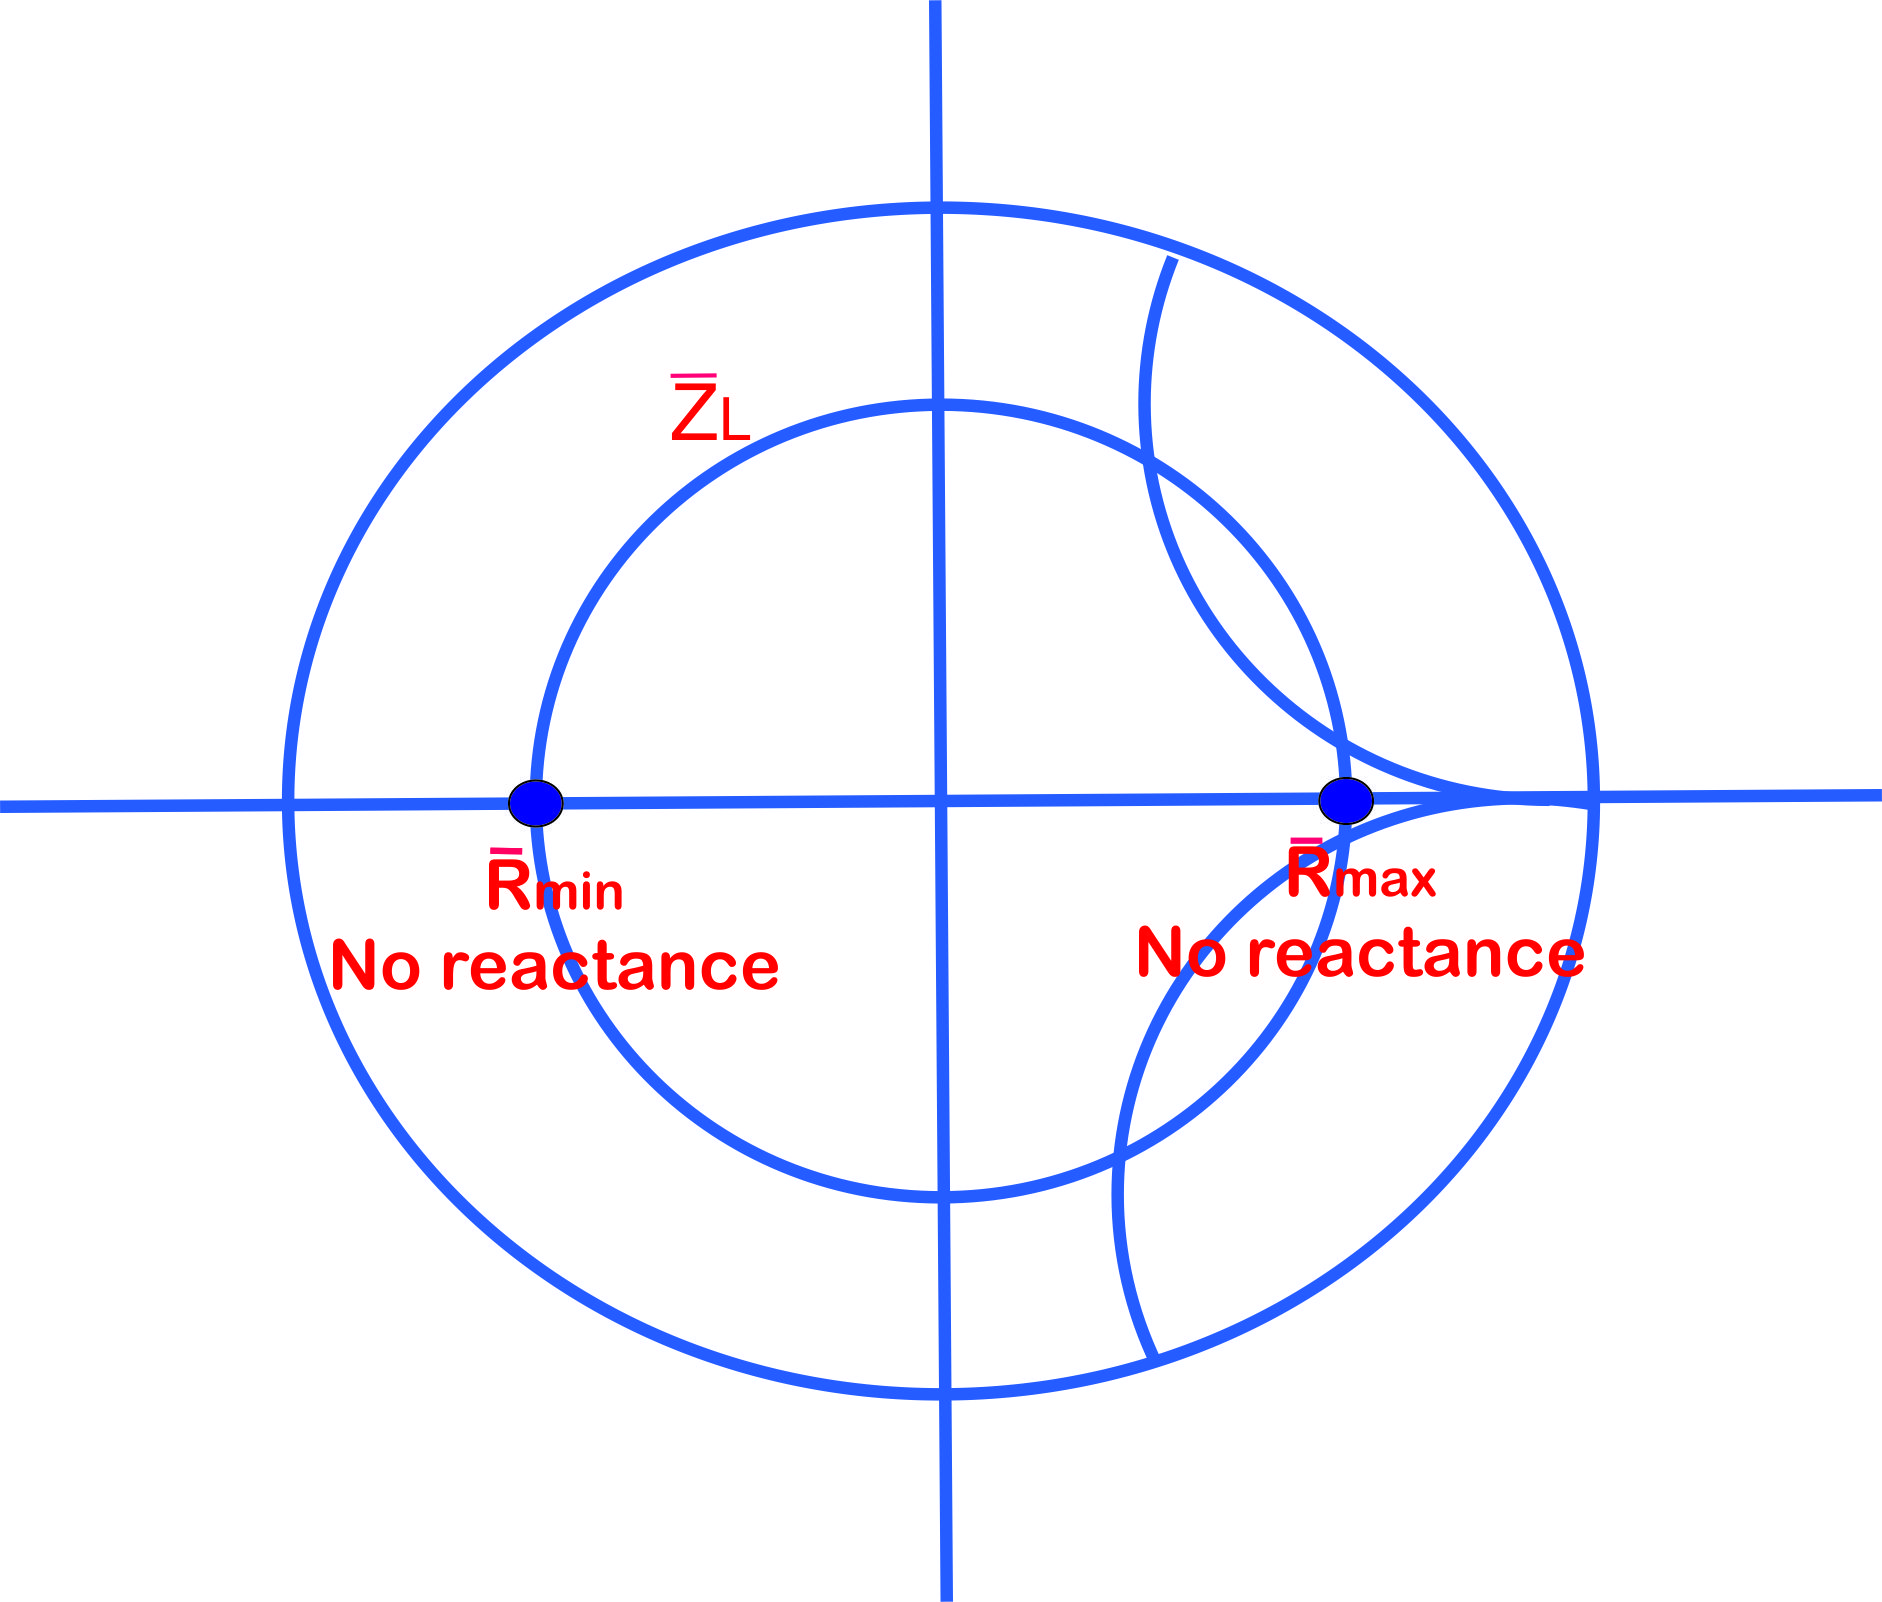
\includegraphics[width=0.7\linewidth]{./graphics/oijhgfdsa}
\caption{Maximum and Minimum Points of Resistance}
\label{fig:oijhgfdsa}
\end{figure}

Hence, the maximum value of the normalized resistance gives VSWR. The maximum value of resistance in terms of normalized quantity is seen when the VSWR circle intersects the real axis on the right side.The rightmost side corresponds to the impedance which is $r_\max$ and the reactance for that is zero\textemdash\;$r_\max$ is nothing but $\rho$. Similarly, the minimum value which we see on transmission line is $r_\min = \frac{1}{\rho}$. The minimum resistance which corresponds to the leftmost intercept on the real axis gives $\frac{1}{\rho}$. Thus once the load impedance or any other impedance is marked on the Smith chart and the constant VSWR circle is drawn, calculation of the VSWR is straightforward same as the reflection coefficient and transformed/normalized impedance. It is just a matter of plotting and reading different values on a Smith chart.

Next is to find out the locations of the  minimum and maximum voltage and current on the transmission line. 

\subsection{Location of the minimum and maximum voltage and current}
Suppose we want to find out the distance of current or voltage maximum at the load end of the transmission line. From our knowledge of transmission line, at point of maximum voltage, we experience minimum current which gives $R_\max$ then at minimum voltage, we experience maximum current which gives $R_\min$ hence $R_\max$ corresponds to $V_\max$,  $I_\min$ and  $R_\min$ corresponds to  $V_\min$, $I_\max$.  To find out these locations from the load, we move from point, $Z_L$ to $r_\max$ and $r_\min$ as shown in figure~\ref{fig:lkjtresx}. The corresponding clockwise angles, $\theta_\max$ and $\theta_\min$, covered indicate the distances $l_\max$ and $l_\min$ towards the generator.
\begin{figure}[h]
\centering
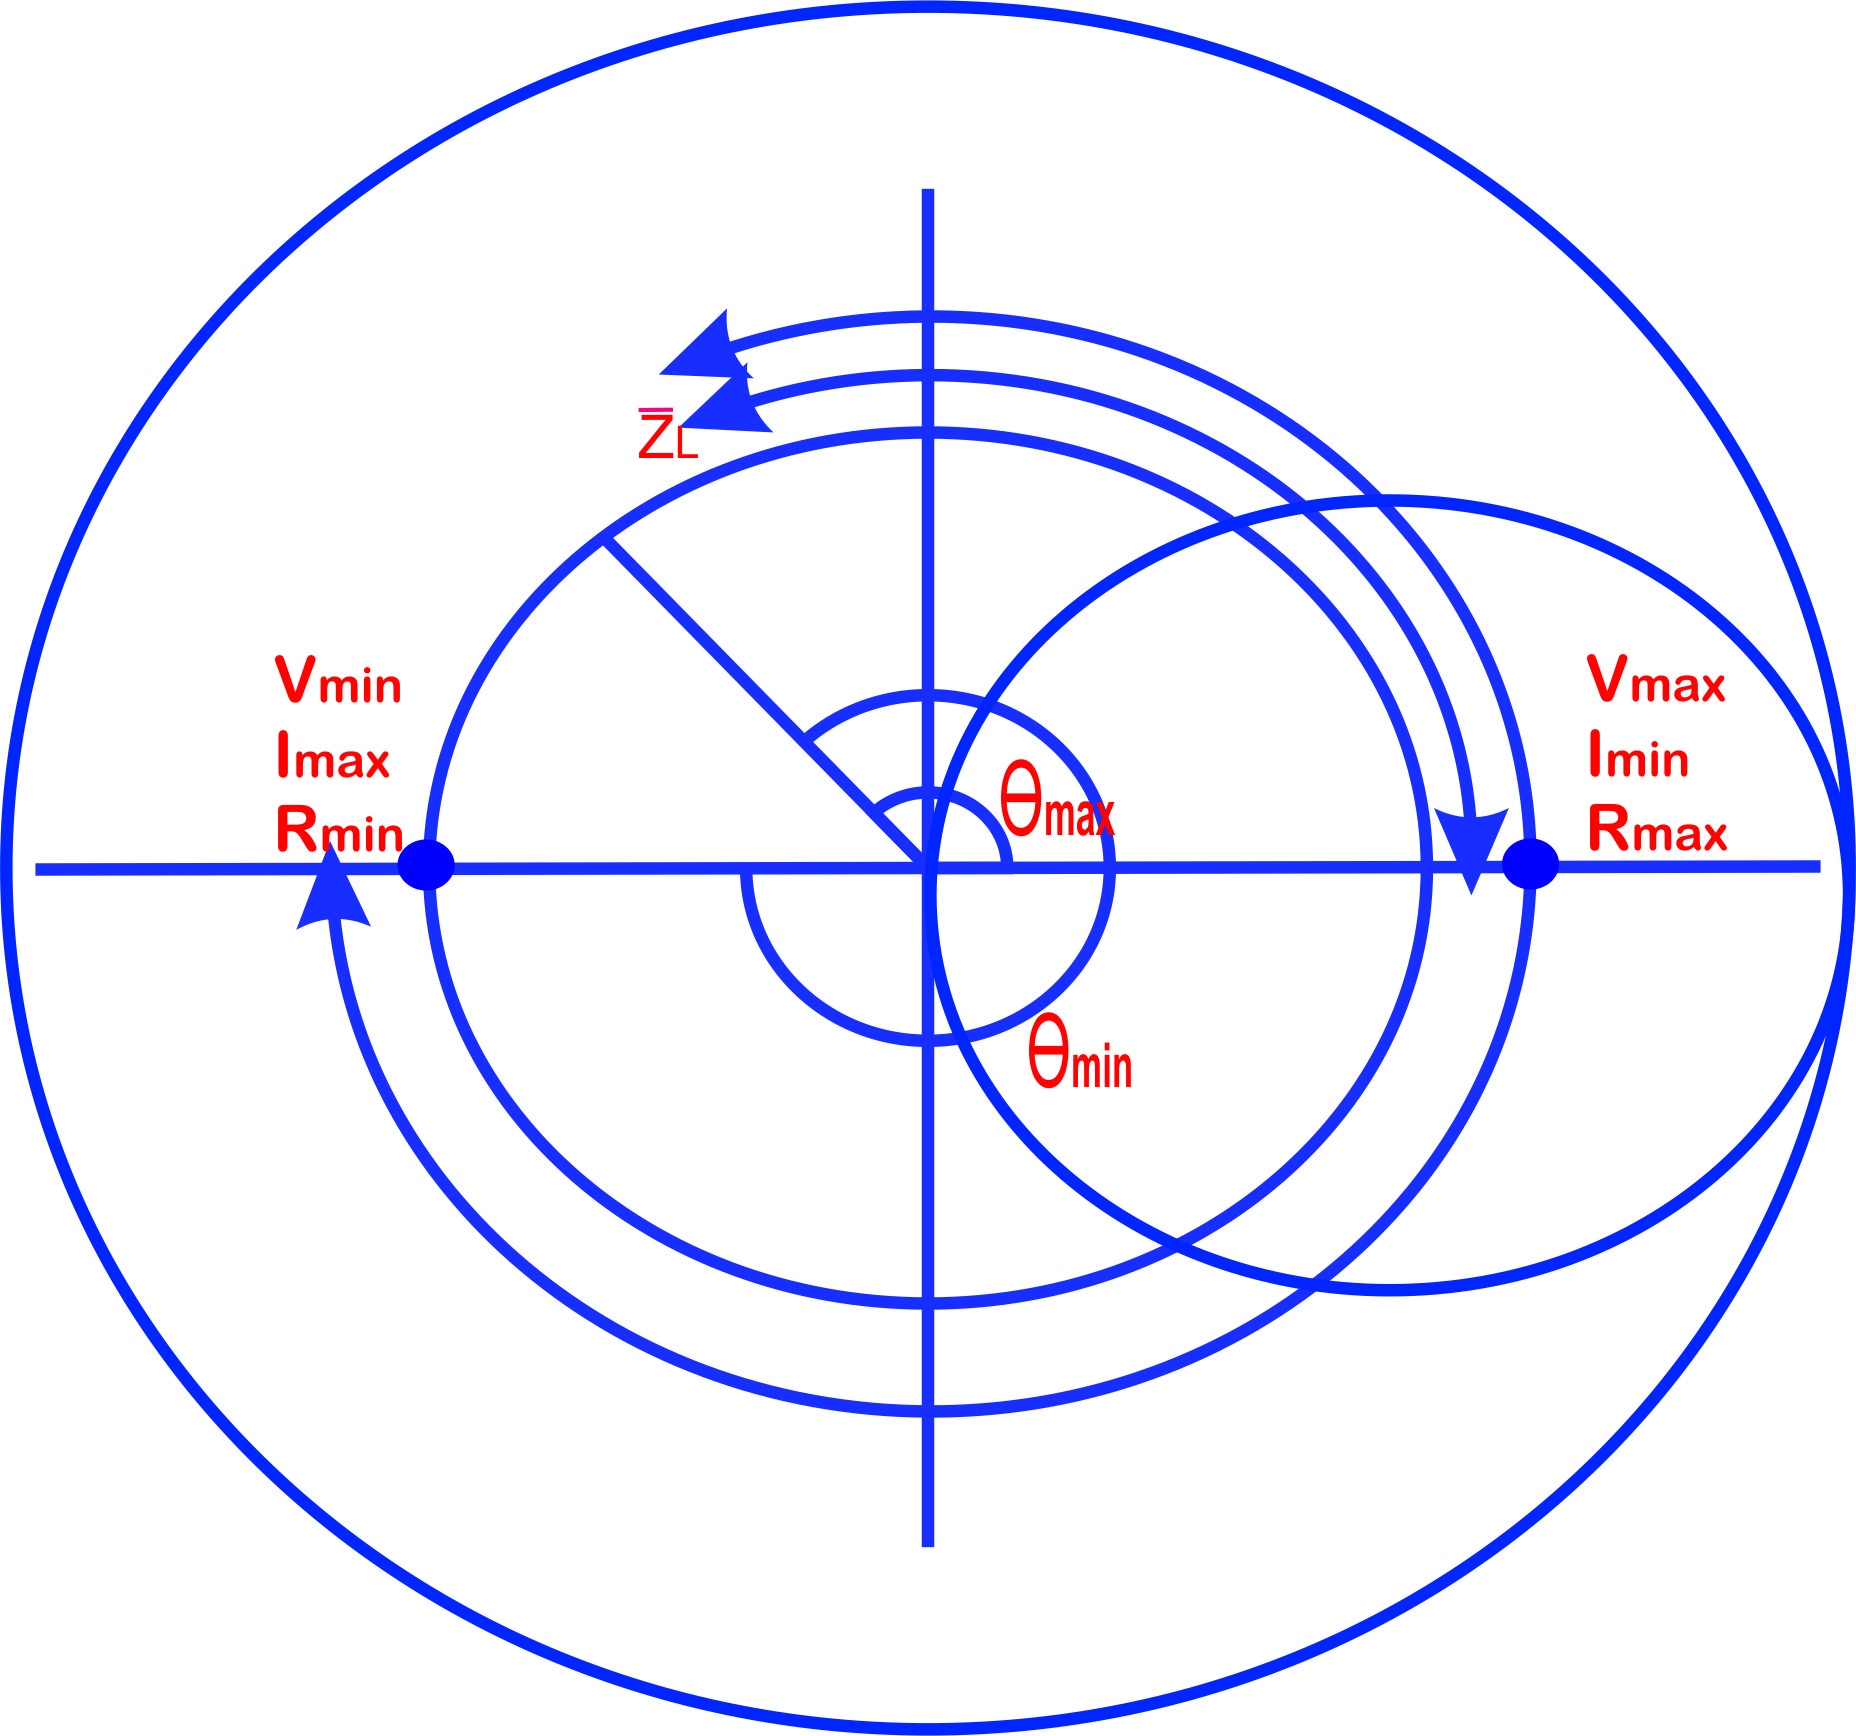
\includegraphics[width=0.7\linewidth]{./graphics/lkjtresx}
\caption{Location of the maximum and minimum values of voltage and current}
\label{fig:lkjtresx}
\end{figure}

We compute the corresponding distances $l_\max$ and $l_\min$, 
recall that $2\beta{l} = \theta\Longrightarrow l =\frac{\theta}{2\beta}$. Hence,
\begin{align*}
l_\max = \frac{\theta_\max}{2\beta}\quad\text{and}\quad l_\min = \frac{\theta_\min}{2\beta}
\end{align*}
These gives the distances from the load point. From figure~\ref{fig:lkjtresx}, $\theta_\max < 180^o(\pi)$ and $270^o\left(\frac{3\pi}{2}\right) <\theta_\min >360^o(2\pi)$ and they therefore are the angles that are moved to get from load to $r_\max$ and $r_\min$ respectively.

More generally,
\begin{dmath}
l = \frac{\theta_\min}{2\beta}
=\frac{\theta_\max + \pi}{2\beta} 
= \frac{\theta_\max}{2\beta} + \frac{\lambda}{4}
\end{dmath}

\begin{exmp}\label{exmp:locatepoints}
\subsubsection*{Locate the points on the Smith chart}
Locate the following points on the Smith chart (Take characteristic impedance, $Z_{0}$ = 50$\Omega$).

\begin{enumerate}[(a)]
\item 50+j75$\varOmega$
\item 10+j0$\varOmega$
\item 0-j80$\varOmega$
\item $\Gamma=0.3\angle60^o$
\item VSWR, $\rho=2.5$
\item $R_\min$ on $\rho$ = 1.5  circle
\end{enumerate}

\subsubsection*{Solution}
All impedances seen on the Smith chart are normalized impedances. Therefore, for impedance (a), (b), and (c), we will first normalize these points with the characteristic impedance such that
\begin{align*}
\bar{A}&=\frac{A}{Z_{0}}
=\frac{50 + j75}{50}\\
&=1+j1.5\\
\bar{B}&=\frac{B}{Z_{0}}
= \frac{10 + j0}{50}\\
&=0.2+j0\\
\bar{C}&=\frac{C}{Z_{0}}
= \frac{0 - j80}{50}\\
&=0-j1.6
\end{align*}

To locate point A on the Smith chart, we first identify the constant resistance circle of $r = 1.0$. It is the circle which passes through the centre of the Smith chart from the right hand side (see figure~\ref{fig:workedexample1}). Next, we identify the constant reactance circle of $x = 1.5$. Recall that the circles above the real axis passing through the centre are the inductive reactance, while the circles below the line are the capacitive reactance. Since the value $x = 1.5$ is positive, it should be the constant inductive reactance circle. The point of intersection of these circle represents the normalized impedance, A, $1 + j1.5$. The same steps applies when identifying points B and C on the Smith chart.
\begin{figure}[h]
\centering
\includegraphics[width=1\linewidth]{"./graphics/Smith chart"}
\caption{Worked Example}
\label{fig:workedexample1}
\end{figure}

To locate point in (d) which is the reflection coefficient, the approach is quite different. First, we measure the length of the diameter of the constant resistance circle $r = 1.0$ and record its value. In our case, we measured $7.6cm$. Thus we can determine the radius of a reflection coefficient of magnitude, $0.3$, that is, by multiplying the length, $7.cm$ with the value of the reflection coefficient which is $0.3$, we will get a value, $2.28cm$. 

Next, we draw a circle of radius $2.28cm$ from the origin on the Smith chart (see figure~\ref{fig:workedexample1}). Note that the degree of rotation (circurmference of the gamma plane\textemdash limit circle) is calibrated in both degrees and distance. To locate the corresponding phase, we look along the circumference showing \textquotedblleft ANGLE OF REFLECTION COEFFICIENT IN DEGREES\textquotedblright\; we will locate the angle 60\textdegree\; anticlockwise. Then draw a straight line through the centre of the plane to the located angle 60\textdegree\; on the Smith chart. The point of intersection of the circle and the line is the point, $\Gamma = 0.3\angle60^o$ on the Smith chart (see figure~\ref{fig:workedexample1}).

To locate point in (e), which is the VSWR of value 2.5, we will locate the point that reads $r = 2.5$ along the real axis on the Smith chart and draw a circle passing through that point from the origin. The VSWR circle of 2.5 is drawn through that point.

To locate point in (f), first, we first draw the VSWR circle of value 1.5 using the steps discussed above. The rightmost side along the circle where the real axis intersects the VSWR circle is the normalized $R_\max$ or $r_\max$ and the leftmost side is the normalized $R_\min$ or $r_\min$. Therefore we record the value at the leftmost side and multiply the value by the characteristic impedance
\begin{align*}
r_\min &= \bar{R}_\min = \frac{R_\min}{Z_0}\\
R_\min  &= \frac{r_\min}{Z_0} = 0.75 \times 50\\
&= 37.5\Omega
\end{align*}
\end{exmp}

\section*{Exercises}
\begin{ExerciseList}
\Exercise[label={ex81}] Locate the following points on the Smith chart for a 70-$\varOmega$ high frequency lossless line.
\begin{enumerate}[(a)]
\item 140 + j91$\varOmega$
\item $\Gamma=0.5\angle29^o$
\item $R_\max$ on $\rho = 3$ circle
\end{enumerate}
\Answer[ref={ex81}]
solution for exercise~\ref{ex81}
\end{ExerciseList}